% DriftAdaptiveForest: documento académico para el Círculo de Ciencia de Datos y Econometría (CCDE).
% Compilar con: latexmk -pdf main.tex   (o en Overleaf, compilador pdfLaTeX + biber)
% Las tablas y las cifras del texto se generan con: python paper/generar_tablas.py
\documentclass[11pt,a4paper]{article}

\usepackage[spanish,es-noshorthands,es-nodecimaldot,es-tabla]{babel}
\usepackage[T1]{fontenc}
\usepackage{lmodern}
\usepackage{microtype}
\usepackage[margin=2.5cm]{geometry}
\usepackage{setspace}\onehalfspacing
\usepackage{csquotes}
\usepackage{amsmath,amssymb}
\usepackage{graphicx}
\usepackage{booktabs,tabularx}
\usepackage{algorithm}
\usepackage{algpseudocode}
\usepackage[hidelinks]{hyperref}
\usepackage[spanish,capitalise,noabbrev]{cleveref}
\usepackage[style=apa,backend=biber]{biblatex}
\addbibresource{referencias.bib}

\floatname{algorithm}{Algoritmo}
\renewcommand{\algorithmicrequire}{\textit{Entrada:}}
\renewcommand{\algorithmicensure}{\textit{Salida:}}
\crefname{algorithm}{Algoritmo}{Algoritmos}
\crefname{table}{Tabla}{Tablas}
\crefname{figure}{Figura}{Figuras}
\crefname{appendix}{Apéndice}{Apéndices}

\setlength{\emergencystretch}{3em}  % evita desbordes por nombres largos en \texttt
\newcommand{\MMD}{\operatorname{MMD}}
\newcommand{\MSE}{\operatorname{MSE}}
\newcommand{\RMSE}{\operatorname{RMSE}}
\newcommand{\nota}[1]{\par\smallskip\raggedright\footnotesize\textit{Nota.} #1}

% Generado por paper/generar_tablas.py. No editar a mano.
\newcommand{\gADFeRealStatic}{3}
\newcommand{\gADFeRealWalk}{2}
\newcommand{\gADFeSintStatic}{8}
\newcommand{\gADFeSintWalk}{10}
\newcommand{\gADFhRealStatic}{3}
\newcommand{\gADFhRealWalk}{1}
\newcommand{\gADFhSintStatic}{8}
\newcommand{\gADFhSintWalk}{9}
\newcommand{\gDRhRealStatic}{1}
\newcommand{\gDRhRealWalk}{0}
\newcommand{\gDRhSintStatic}{6}
\newcommand{\gDRhSintWalk}{6}
\newcommand{\gDRmRealStatic}{3}
\newcommand{\gDRmRealWalk}{2}
\newcommand{\gDRmSintStatic}{4}
\newcommand{\gDRmSintWalk}{5}
\newcommand{\gDRrRealStatic}{2}
\newcommand{\gDRrRealWalk}{1}
\newcommand{\gDRrSintStatic}{6}
\newcommand{\gDRrSintWalk}{6}
\newcommand{\gDRrefitRealStatic}{2}
\newcommand{\gDRrefitRealWalk}{1}
\newcommand{\gDRrefitSintStatic}{7}
\newcommand{\gDRrefitSintWalk}{9}
\newcommand{\gRFERealStatic}{2}
\newcommand{\gRFERealWalk}{2}
\newcommand{\gRFESintStatic}{7}
\newcommand{\gRFESintWalk}{8}
\newcommand{\gRFVRealStatic}{2}
\newcommand{\gRFVRealWalk}{1}
\newcommand{\gRFVSintStatic}{7}
\newcommand{\gRFVSintWalk}{7}
\newcommand{\gasDRmax}{1.89}
\newcommand{\gasDRmin}{1.43}
\newcommand{\hCuatroConceptGeo}{0.750}
\newcommand{\hCuatroSinMax}{1.00}
\newcommand{\hCuatroVsRFV}{8}
\newcommand{\hDosMax}{1.19}
\newcommand{\hDosMin}{1.18}
\newcommand{\hTresN}{11}
\newcommand{\hTresRFE}{5}
\newcommand{\hTresRFV}{9}
\newcommand{\hUnoGana}{6}
\newcommand{\hUnoGeo}{0.917}
\newcommand{\kADFeRealStatic}{2.80}
\newcommand{\kADFeRealWalk}{3.00}
\newcommand{\kADFeSintStatic}{2.73}
\newcommand{\kADFeSintWalk}{2.00}
\newcommand{\kADFhRealStatic}{3.40}
\newcommand{\kADFhRealWalk}{4.40}
\newcommand{\kADFhSintStatic}{2.55}
\newcommand{\kADFhSintWalk}{2.82}
\newcommand{\kDRhRealStatic}{8.40}
\newcommand{\kDRhRealWalk}{6.40}
\newcommand{\kDRhSintStatic}{6.91}
\newcommand{\kDRhSintWalk}{7.18}
\newcommand{\kDRmRealStatic}{4.40}
\newcommand{\kDRmRealWalk}{4.20}
\newcommand{\kDRmSintStatic}{7.00}
\newcommand{\kDRmSintWalk}{6.91}
\newcommand{\kDRrRealStatic}{5.60}
\newcommand{\kDRrRealWalk}{7.40}
\newcommand{\kDRrSintStatic}{6.45}
\newcommand{\kDRrSintWalk}{6.55}
\newcommand{\kDRrefitRealStatic}{4.00}
\newcommand{\kDRrefitRealWalk}{5.80}
\newcommand{\kDRrefitSintStatic}{4.36}
\newcommand{\kDRrefitSintWalk}{4.36}
\newcommand{\kRFERealStatic}{5.60}
\newcommand{\kRFERealWalk}{4.40}
\newcommand{\kRFESintStatic}{5.27}
\newcommand{\kRFESintWalk}{5.09}
\newcommand{\kRFRealStatic}{4.60}
\newcommand{\kRFRealWalk}{3.40}
\newcommand{\kRFSintStatic}{5.91}
\newcommand{\kRFSintWalk}{6.09}
\newcommand{\kRFVRealStatic}{6.20}
\newcommand{\kRFVRealWalk}{6.00}
\newcommand{\kRFVSintStatic}{3.82}
\newcommand{\kRFVSintWalk}{4.00}
\newcommand{\nConcept}{8}
\newcommand{\optBothDR}{3.02}
\newcommand{\optBothDRpct}{51.5}
\newcommand{\optBothRF}{6.22}
\newcommand{\optBothRFV}{2.16}
\newcommand{\optBothRFVpct}{65.2}
\newcommand{\optDRganaRF}{3}
\newcommand{\optGasDRpct}{56.5}
\newcommand{\optN}{10}
\newcommand{\optRFVganaDR}{9}
\newcommand{\pADFeRealStatic}{0.312}
\newcommand{\pADFeRealWalk}{1.000}
\newcommand{\pADFeSintStatic}{0.042}
\newcommand{\pADFeSintWalk}{0.002}
\newcommand{\pADFhRealStatic}{0.625}
\newcommand{\pADFhRealWalk}{0.625}
\newcommand{\pADFhSintStatic}{0.014}
\newcommand{\pADFhSintWalk}{0.010}
\newcommand{\pDRhRealStatic}{0.125}
\newcommand{\pDRhRealWalk}{0.062}
\newcommand{\pDRhSintStatic}{0.638}
\newcommand{\pDRhSintWalk}{1.000}
\newcommand{\pDRmRealStatic}{0.812}
\newcommand{\pDRmRealWalk}{0.625}
\newcommand{\pDRmSintStatic}{0.320}
\newcommand{\pDRmSintWalk}{0.240}
\newcommand{\pDRrRealStatic}{1.000}
\newcommand{\pDRrRealWalk}{0.438}
\newcommand{\pDRrSintStatic}{0.278}
\newcommand{\pDRrSintWalk}{0.465}
\newcommand{\pDRrefitRealStatic}{1.000}
\newcommand{\pDRrefitRealWalk}{0.625}
\newcommand{\pDRrefitSintStatic}{0.175}
\newcommand{\pDRrefitSintWalk}{0.054}
\newcommand{\pRFERealStatic}{0.312}
\newcommand{\pRFERealWalk}{1.000}
\newcommand{\pRFESintStatic}{0.042}
\newcommand{\pRFESintWalk}{0.014}
\newcommand{\pRFVRealStatic}{0.812}
\newcommand{\pRFVRealWalk}{0.438}
\newcommand{\pRFVSintStatic}{0.083}
\newcommand{\pRFVSintWalk}{0.067}
\newcommand{\peorDRsinConcept}{29}
\newcommand{\rADFeRealStatic}{0.919}
\newcommand{\rADFeRealWalk}{0.983}
\newcommand{\rADFeSintStatic}{0.698}
\newcommand{\rADFeSintWalk}{0.809}
\newcommand{\rADFhRealStatic}{0.955}
\newcommand{\rADFhRealWalk}{1.004}
\newcommand{\rADFhSintStatic}{0.683}
\newcommand{\rADFhSintWalk}{0.821}
\newcommand{\rDRhRealStatic}{1.209}
\newcommand{\rDRhRealWalk}{1.088}
\newcommand{\rDRhSintStatic}{0.940}
\newcommand{\rDRhSintWalk}{1.008}
\newcommand{\rDRmRealStatic}{1.038}
\newcommand{\rDRmRealWalk}{1.020}
\newcommand{\rDRmSintStatic}{1.019}
\newcommand{\rDRmSintWalk}{1.036}
\newcommand{\rDRrRealStatic}{0.990}
\newcommand{\rDRrRealWalk}{1.073}
\newcommand{\rDRrSintStatic}{0.897}
\newcommand{\rDRrSintWalk}{0.965}
\newcommand{\rDRrefitRealStatic}{0.961}
\newcommand{\rDRrefitRealWalk}{1.034}
\newcommand{\rDRrefitSintStatic}{0.768}
\newcommand{\rDRrefitSintWalk}{0.873}
\newcommand{\rRFERealStatic}{1.024}
\newcommand{\rRFERealWalk}{1.002}
\newcommand{\rRFESintStatic}{0.902}
\newcommand{\rRFESintWalk}{0.936}
\newcommand{\rRFVRealStatic}{1.004}
\newcommand{\rRFVRealWalk}{1.049}
\newcommand{\rRFVSintStatic}{0.699}
\newcommand{\rRFVSintWalk}{0.839}
\newcommand{\wADFeRealStatic}{60}
\newcommand{\wADFeRealWalk}{57}
\newcommand{\wADFeSintStatic}{79}
\newcommand{\wADFeSintWalk}{81}
\newcommand{\wADFhRealStatic}{60}
\newcommand{\wADFhRealWalk}{50}
\newcommand{\wADFhSintStatic}{79}
\newcommand{\wADFhSintWalk}{73}
\newcommand{\wDRhRealStatic}{20}
\newcommand{\wDRhRealWalk}{23}
\newcommand{\wDRhSintStatic}{45}
\newcommand{\wDRhSintWalk}{33}
\newcommand{\wDRmRealStatic}{60}
\newcommand{\wDRmRealWalk}{40}
\newcommand{\wDRmSintStatic}{33}
\newcommand{\wDRmSintWalk}{37}
\newcommand{\wDRrRealStatic}{40}
\newcommand{\wDRrRealWalk}{27}
\newcommand{\wDRrSintStatic}{52}
\newcommand{\wDRrSintWalk}{40}
\newcommand{\wDRrefitRealStatic}{40}
\newcommand{\wDRrefitRealWalk}{33}
\newcommand{\wDRrefitSintStatic}{64}
\newcommand{\wDRrefitSintWalk}{57}
\newcommand{\wRFERealStatic}{40}
\newcommand{\wRFERealWalk}{60}
\newcommand{\wRFESintStatic}{67}
\newcommand{\wRFESintWalk}{68}
\newcommand{\wRFVRealStatic}{40}
\newcommand{\wRFVRealWalk}{37}
\newcommand{\wRFVSintStatic}{67}
\newcommand{\wRFVSintWalk}{54}
\newcommand{\xADFeAirQualityStatic}{0.90}
\newcommand{\xADFeAirQualityWalk}{1.04}
\newcommand{\xADFeBeijingPmStatic}{0.97}
\newcommand{\xADFeBeijingPmWalk}{0.98}
\newcommand{\xADFeBikeSharingStatic}{0.74}
\newcommand{\xADFeBikeSharingWalk}{0.85}
\newcommand{\xADFeCovariateShiftStatic}{1.00}
\newcommand{\xADFeCovariateShiftWalk}{0.98}
\newcommand{\xADFeElectricityStatic}{1.01}
\newcommand{\xADFeElectricityWalk}{1.05}
\newcommand{\xADFeFriedmanAbruptStatic}{0.62}
\newcommand{\xADFeFriedmanAbruptWalk}{0.83}
\newcommand{\xADFeFriedmanGradualDataStatic}{0.92}
\newcommand{\xADFeFriedmanGradualDataWalk}{0.93}
\newcommand{\xADFeFriedmanRecurringStatic}{1.02}
\newcommand{\xADFeFriedmanRecurringWalk}{0.97}
\newcommand{\xADFeGasDriftStatic}{1.00}
\newcommand{\xADFeGasDriftWalk}{1.00}
\newcommand{\xADFeHealthcareBothStatic}{0.29}
\newcommand{\xADFeHealthcareBothWalk}{0.53}
\newcommand{\xADFeHealthcareConceptStatic}{0.31}
\newcommand{\xADFeHealthcareConceptWalk}{0.52}
\newcommand{\xADFeHealthcareDataStatic}{0.98}
\newcommand{\xADFeHealthcareDataWalk}{1.00}
\newcommand{\xADFeHealthcareNoneStatic}{0.97}
\newcommand{\xADFeHealthcareNoneWalk}{0.98}
\newcommand{\xADFeHighdimMixedStatic}{1.09}
\newcommand{\xADFeHighdimMixedWalk}{0.96}
\newcommand{\xADFeIncrementalStatic}{0.67}
\newcommand{\xADFeIncrementalWalk}{0.72}
\newcommand{\xADFeLocalDriftStatic}{0.52}
\newcommand{\xADFeLocalDriftWalk}{0.72}
\newcommand{\xDRhAirQualityStatic}{0.98}
\newcommand{\xDRhAirQualityWalk}{1.03}
\newcommand{\xDRhBeijingPmStatic}{1.09}
\newcommand{\xDRhBeijingPmWalk}{1.06}
\newcommand{\xDRhBikeSharingStatic}{1.03}
\newcommand{\xDRhBikeSharingWalk}{1.05}
\newcommand{\xDRhCovariateShiftStatic}{1.23}
\newcommand{\xDRhCovariateShiftWalk}{1.19}
\newcommand{\xDRhElectricityStatic}{1.23}
\newcommand{\xDRhElectricityWalk}{1.06}
\newcommand{\xDRhFriedmanAbruptStatic}{0.87}
\newcommand{\xDRhFriedmanAbruptWalk}{0.99}
\newcommand{\xDRhFriedmanGradualDataStatic}{1.18}
\newcommand{\xDRhFriedmanGradualDataWalk}{1.10}
\newcommand{\xDRhFriedmanRecurringStatic}{0.72}
\newcommand{\xDRhFriedmanRecurringWalk}{0.82}
\newcommand{\xDRhGasDriftStatic}{1.89}
\newcommand{\xDRhGasDriftWalk}{1.26}
\newcommand{\xDRhHealthcareBothStatic}{0.85}
\newcommand{\xDRhHealthcareBothWalk}{0.95}
\newcommand{\xDRhHealthcareConceptStatic}{0.76}
\newcommand{\xDRhHealthcareConceptWalk}{0.95}
\newcommand{\xDRhHealthcareDataStatic}{1.16}
\newcommand{\xDRhHealthcareDataWalk}{1.29}
\newcommand{\xDRhHealthcareNoneStatic}{1.01}
\newcommand{\xDRhHealthcareNoneWalk}{1.04}
\newcommand{\xDRhHighdimMixedStatic}{1.34}
\newcommand{\xDRhHighdimMixedWalk}{1.10}
\newcommand{\xDRhIncrementalStatic}{1.00}
\newcommand{\xDRhIncrementalWalk}{0.88}
\newcommand{\xDRhLocalDriftStatic}{0.55}
\newcommand{\xDRhLocalDriftWalk}{0.89}
\newcommand{\xDRmAirQualityStatic}{0.94}
\newcommand{\xDRmAirQualityWalk}{1.03}
\newcommand{\xDRmBeijingPmStatic}{1.01}
\newcommand{\xDRmBeijingPmWalk}{0.99}
\newcommand{\xDRmBikeSharingStatic}{0.98}
\newcommand{\xDRmBikeSharingWalk}{1.01}
\newcommand{\xDRmCovariateShiftStatic}{1.17}
\newcommand{\xDRmCovariateShiftWalk}{1.19}
\newcommand{\xDRmElectricityStatic}{0.91}
\newcommand{\xDRmElectricityWalk}{0.91}
\newcommand{\xDRmFriedmanAbruptStatic}{0.99}
\newcommand{\xDRmFriedmanAbruptWalk}{1.04}
\newcommand{\xDRmFriedmanGradualDataStatic}{1.02}
\newcommand{\xDRmFriedmanGradualDataWalk}{1.04}
\newcommand{\xDRmFriedmanRecurringStatic}{1.01}
\newcommand{\xDRmFriedmanRecurringWalk}{0.98}
\newcommand{\xDRmGasDriftStatic}{1.43}
\newcommand{\xDRmGasDriftWalk}{1.17}
\newcommand{\xDRmHealthcareBothStatic}{0.89}
\newcommand{\xDRmHealthcareBothWalk}{0.92}
\newcommand{\xDRmHealthcareConceptStatic}{1.00}
\newcommand{\xDRmHealthcareConceptWalk}{0.99}
\newcommand{\xDRmHealthcareDataStatic}{1.12}
\newcommand{\xDRmHealthcareDataWalk}{1.18}
\newcommand{\xDRmHealthcareNoneStatic}{0.98}
\newcommand{\xDRmHealthcareNoneWalk}{0.99}
\newcommand{\xDRmHighdimMixedStatic}{1.05}
\newcommand{\xDRmHighdimMixedWalk}{1.08}
\newcommand{\xDRmIncrementalStatic}{0.99}
\newcommand{\xDRmIncrementalWalk}{1.00}
\newcommand{\xDRmLocalDriftStatic}{1.01}
\newcommand{\xDRmLocalDriftWalk}{1.02}
\newcommand{\xDRrAirQualityStatic}{0.92}
\newcommand{\xDRrAirQualityWalk}{1.06}
\newcommand{\xDRrBeijingPmStatic}{1.06}
\newcommand{\xDRrBeijingPmWalk}{1.08}
\newcommand{\xDRrBikeSharingStatic}{0.63}
\newcommand{\xDRrBikeSharingWalk}{0.88}
\newcommand{\xDRrCovariateShiftStatic}{1.25}
\newcommand{\xDRrCovariateShiftWalk}{1.19}
\newcommand{\xDRrElectricityStatic}{1.04}
\newcommand{\xDRrElectricityWalk}{1.13}
\newcommand{\xDRrFriedmanAbruptStatic}{0.74}
\newcommand{\xDRrFriedmanAbruptWalk}{0.94}
\newcommand{\xDRrFriedmanGradualDataStatic}{1.18}
\newcommand{\xDRrFriedmanGradualDataWalk}{1.11}
\newcommand{\xDRrFriedmanRecurringStatic}{1.13}
\newcommand{\xDRrFriedmanRecurringWalk}{0.98}
\newcommand{\xDRrGasDriftStatic}{1.50}
\newcommand{\xDRrGasDriftWalk}{1.25}
\newcommand{\xDRrHealthcareBothStatic}{0.76}
\newcommand{\xDRrHealthcareBothWalk}{0.86}
\newcommand{\xDRrHealthcareConceptStatic}{0.62}
\newcommand{\xDRrHealthcareConceptWalk}{0.78}
\newcommand{\xDRrHealthcareDataStatic}{1.11}
\newcommand{\xDRrHealthcareDataWalk}{1.13}
\newcommand{\xDRrHealthcareNoneStatic}{0.99}
\newcommand{\xDRrHealthcareNoneWalk}{1.01}
\newcommand{\xDRrHighdimMixedStatic}{1.10}
\newcommand{\xDRrHighdimMixedWalk}{1.07}
\newcommand{\xDRrIncrementalStatic}{0.80}
\newcommand{\xDRrIncrementalWalk}{0.83}
\newcommand{\xDRrLocalDriftStatic}{0.54}
\newcommand{\xDRrLocalDriftWalk}{0.83}
\newcommand{\xRFVAirQualityStatic}{0.98}
\newcommand{\xRFVAirQualityWalk}{1.08}
\newcommand{\xRFVBeijingPmStatic}{1.14}
\newcommand{\xRFVBeijingPmWalk}{1.20}
\newcommand{\xRFVBikeSharingStatic}{0.72}
\newcommand{\xRFVBikeSharingWalk}{0.86}
\newcommand{\xRFVCovariateShiftStatic}{1.08}
\newcommand{\xRFVCovariateShiftWalk}{1.08}
\newcommand{\xRFVElectricityStatic}{1.07}
\newcommand{\xRFVElectricityWalk}{1.03}
\newcommand{\xRFVFriedmanAbruptStatic}{0.56}
\newcommand{\xRFVFriedmanAbruptWalk}{0.82}
\newcommand{\xRFVFriedmanGradualDataStatic}{0.93}
\newcommand{\xRFVFriedmanGradualDataWalk}{0.93}
\newcommand{\xRFVFriedmanRecurringStatic}{1.15}
\newcommand{\xRFVFriedmanRecurringWalk}{1.02}
\newcommand{\xRFVGasDriftStatic}{1.20}
\newcommand{\xRFVGasDriftWalk}{1.11}
\newcommand{\xRFVHealthcareBothStatic}{0.32}
\newcommand{\xRFVHealthcareBothWalk}{0.57}
\newcommand{\xRFVHealthcareConceptStatic}{0.36}
\newcommand{\xRFVHealthcareConceptWalk}{0.57}
\newcommand{\xRFVHealthcareDataStatic}{1.03}
\newcommand{\xRFVHealthcareDataWalk}{1.11}
\newcommand{\xRFVHealthcareNoneStatic}{1.08}
\newcommand{\xRFVHealthcareNoneWalk}{1.07}
\newcommand{\xRFVHighdimMixedStatic}{0.71}
\newcommand{\xRFVHighdimMixedWalk}{0.90}
\newcommand{\xRFVIncrementalStatic}{0.67}
\newcommand{\xRFVIncrementalWalk}{0.72}
\newcommand{\xRFVLocalDriftStatic}{0.50}
\newcommand{\xRFVLocalDriftWalk}{0.70}


\title{Bosques aleatorios adaptativos al drift:\\ ensambles por ventanas temporales para regresión no estacionaria}
\author{Mauricio Aguirre Stornaiuolo \and Piero Alexander Simeon Bustillos\\[4pt]
  \small Círculo de Ciencia de Datos y Econometría (CCDE)}
\date{Noviembre de 2026}

\begin{document}

\begin{titlepage}
  \centering
  
\includegraphics[width=0.28\textwidth]{logo_ccde.jpeg}\par\vspace{1.5cm}
  {\LARGE Bosques aleatorios adaptativos al drift:\par}
  \vspace{0.3cm}
  {\Large ensambles por ventanas temporales para regresión no estacionaria\par}
  \vspace{1.5cm}
  {\large Mauricio Aguirre Stornaiuolo\par Piero Alexander Simeon Bustillos\par}
  \vspace{1cm}
  {\large Círculo de Ciencia de Datos y Econometría (CCDE)\par}
  \vspace{0.5cm}
  {Documento de trabajo\par Noviembre de 2026\par}
  \vfill
  \begin{minipage}{0.9\textwidth}
    \footnotesize\raggedright
    \copyright{} 2026 CCDE. Todos los derechos
    reservados. El texto, el código fuente (\texttt{DriftAdaptiveForest}) y los modelos
    \texttt{DriftRegressor} y \texttt{AdaptiveDriftForest} descritos en este documento se distribuyen
    bajo una licencia de código visible con uso bajo autorización (archivo \texttt{LICENSE} del
    repositorio \url{https://github.com/CCDE-DataLab/DriftAdaptiveForest}). Cualquier persona puede
    leerlos y citarlos; su uso, reproducción, distribución o explotación comercial requieren
    contactar a los autores y obtener su autorización escrita.
  \end{minipage}
\end{titlepage}

\begin{abstract}
\noindent Un bosque aleatorio entrenado con todo el histórico promedia regímenes que ya no rigen cuando
cambia la distribución de las covariables (data drift) o la relación entre covariables y objetivo
(concept drift). Este trabajo evalúa dos ensambles de bosques aleatorios para regresión temporal: el
\texttt{DriftRegressor}, que entrena un sub-bosque por bloque temporal y los pondera por discrepancia
de media máxima (MMD) o por error reciente, y el \texttt{AdaptiveDriftForest}, una versión rediseñada a
partir del diagnóstico del primero que añade ventanas recientes anidadas, penalización por error
normalizado y reentrenamiento con los datos más recientes. La evaluación usa 11 escenarios sintéticos
y 5 conjuntos de datos reales con drift documentado, dos protocolos temporales (partición 80/20 y
walk-forward con ventana expansiva) y, como líneas base, un bosque aleatorio con todo el histórico, uno
con el 20\,\% más reciente y uno con pesos exponenciales. El \texttt{DriftRegressor} solo mejora al
bosque convencional bajo concept drift, empeora hasta en \peorDRsinConcept\,\% cuando solo hay data
drift, y es superado por la ventana reciente en \hTresRFV{} de \hTresN{} escenarios. El
\texttt{AdaptiveDriftForest} reduce el RMSE de walk-forward en los escenarios sintéticos a
\rADFeSintWalk{} veces el del bosque convencional (\gADFeSintWalk{} de 11 escenarios, Wilcoxon
$p=\pADFeSintWalk$) y a \rADFeRealWalk{} en los datos reales, donde la diferencia no es
estadísticamente distinguible con cinco conjuntos. La comparación contra líneas base de recencia
resulta indispensable para evaluar cualquier método adaptativo al drift.
\end{abstract}

\noindent\textit{Palabras clave:} concept drift, data drift, bosques aleatorios, ensambles temporales,
discrepancia de media máxima, validación walk-forward.

\newpage
\tableofcontents
\newpage

% =====================================================================================
\section{Introducción}\label{sec:intro}

En el conjunto sintético de estancias hospitalarias que motivó este proyecto, un cambio de protocolo
clínico alrededor del 60\,\% de la muestra altera la relación entre la severidad del paciente y los
días de estancia. Un bosque aleatorio (RF) entrenado con los primeros 4\,000 ingresos obtiene un RMSE
de 6.40 días sobre los 1\,000 siguientes. En promedio sobre tres réplicas del mismo escenario, un RF
entrenado solo con el 20\,\% más reciente del histórico tiene un error de \xRFVHealthcareBothStatic{}
veces el del RF con todo el histórico (\cref{tab:sint-static}). La diferencia no viene de la
capacidad del modelo, sino de qué datos se le dan.

La \cref{fig:motivacion} muestra los dos cambios que ocurren en ese escenario. En el panel (a), la
severidad media de los pacientes que ingresan sube y oscila con el tiempo: cambia el tipo de paciente
que llega. En el panel (b), para una misma severidad, los días de estancia dependen de la época: con
el protocolo antiguo la estancia apenas responde a la severidad, mientras que con el nuevo crece casi
en línea recta. Un modelo entrenado con todo el histórico aprende un promedio de ambas reglas, que no
describe ninguna de las dos.

\begin{figure}[htbp]
  \centering
  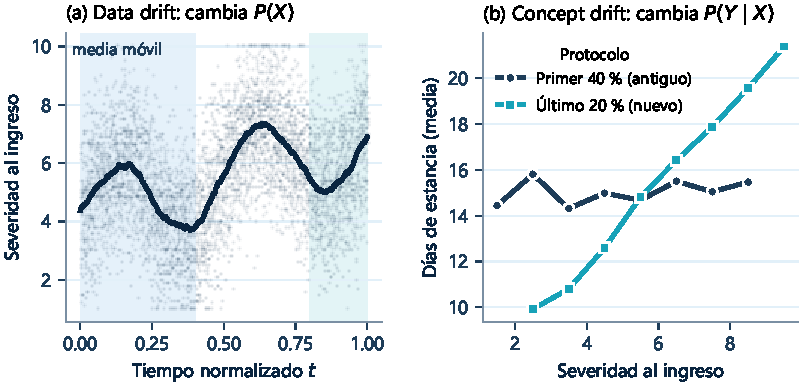
\includegraphics[width=\textwidth]{figuras/motivacion_drift.pdf}
  \caption{Los dos tipos de drift en el escenario hospitalario}\label{fig:motivacion}
  \nota{(a) Severidad al ingreso de cada paciente (puntos) y su media móvil de 250 ingresos (línea);
  las bandas marcan el primer 40\,\% y el último 20\,\% de la muestra. (b) Días de estancia medios por
  intervalo de severidad en esos dos tramos (intervalos con al menos 15 pacientes). \textit{Fuente:}
  \texttt{data/raw/healthcare\_both\_drift.parquet}, generado con \texttt{generate\_data.py}.}
\end{figure}

El mismo problema aparece en muchos contextos aplicados. Un modelo de riesgo crediticio entrenado en
un periodo de tasas bajas puede asignar a un mismo perfil de cliente una probabilidad de mora que deja
de ser válida cuando la política monetaria se endurece. Un modelo de demanda de un comercio minorista
aprende patrones de compra que cambian tras un evento como una pandemia o la llegada de un canal
digital. Un sensor químico se degrada con los meses y su lectura deja de corresponder a la misma
concentración, que es el caso de dos de los conjuntos reales de este trabajo. En un mercado eléctrico,
un cambio regulatorio altera la relación entre precio y demanda. En econometría el fenómeno tiene un
nombre conocido, el cambio estructural: los parámetros de la relación entre variables cambian en
fechas desconocidas, y existe una tradición de pruebas para detectarlo
\parencite{andrews1993,baiperron1998}. La diferencia en aprendizaje automático es que la relación no
es lineal ni paramétrica, y que el objetivo no es fechar el quiebre, sino predecir bien después de
él.

Este fenómeno se conoce como drift. La literatura distingue el cambio en la distribución de las
covariables, $P(X)$, llamado data drift o covariate shift, del cambio en la distribución condicional
$P(Y\mid X)$, llamado concept drift \parencite{gama2014,morenotorres2012}. Un RF clásico
\parencite{breiman2001} enfrenta ambos con dos limitaciones: el muestreo bootstrap uniforme mezcla
observaciones de todas las épocas en cada árbol, y los árboles no extrapolan fuera del rango
observado ni distinguen regímenes que asignan respuestas distintas a una misma región de $X$.

La respuesta habitual de la literatura de flujos de datos es el ensamble de modelos entrenados en
distintos tramos del pasado, con pesos que se actualizan según su desempeño reciente
\parencite{kolter2007,elwell2011,gomes2017}. Esa literatura se concentra en clasificación y en
aprendizaje en línea. En regresión por lotes, que es el caso típico de un analista que reentrena un
modelo cada cierto tiempo, la pregunta práctica es más simple: dado un histórico ordenado en el
tiempo, ¿qué subconjunto o qué combinación de modelos entrenados en ese histórico predice mejor el
futuro inmediato?

Este documento responde esa pregunta para dos propuestas desarrolladas en el CCDE. La primera, el
\texttt{DriftRegressor}, divide el histórico en $K$ bloques, entrena un RF por bloque y combina sus
predicciones con pesos que penalizan la distancia MMD \parencite{gretton2012} entre cada bloque y los
datos a predecir, el error del bloque sobre el tramo más reciente o ambas. La segunda, el
\texttt{AdaptiveDriftForest}, se diseñó después de evaluar la primera y corrige los problemas que esa
evaluación encontró.

La pregunta general es si un ensamble de bosques ponderado por bloques temporales predice mejor que
un RF convencional y que las líneas base triviales de recencia cuando hay drift. Las preguntas
específicas son: (P1) ¿mejora el \texttt{DriftRegressor} al RF convencional bajo concept drift?; (P2)
¿lo mejora cuando solo hay data drift?; (P3) ¿su ventaja proviene de la ponderación por bloques o
basta con entrenar con datos recientes?; y (P4) ¿corrige el \texttt{AdaptiveDriftForest} las
debilidades encontradas sin perder frente al RF cuando no hay drift?

Los resultados principales son tres. El \texttt{DriftRegressor} mejora al RF convencional solo cuando
hay concept drift y empeora cuando solo hay data drift. Un RF entrenado con el 20\,\% más reciente del
histórico lo supera en la mayoría de escenarios, lo que indica que gran parte de la ganancia atribuida
a la ponderación por bloques es un efecto de recencia. El \texttt{AdaptiveDriftForest}, que incluye
esas ventanas recientes entre sus candidatos, es el modelo con mejor rango medio en los cuatro cortes
evaluados, con una ventaja clara en los datos sintéticos y modesta en los reales. El aporte del
trabajo es metodológico: un protocolo de evaluación temporal con líneas base de recencia y un
diagnóstico de drift independiente de los modelos, que cambia la lectura de los resultados
publicados en la primera versión del repositorio.

% =====================================================================================
\section{Marco teórico}\label{sec:marco}

\subsection{Tipos de drift}

Sea $(X_t, Y_t)$ un proceso con distribución conjunta $P_t(X,Y) = P_t(X)\,P_t(Y\mid X)$. Hay drift
entre los instantes $t$ y $t'$ cuando $P_t(X,Y)\neq P_{t'}(X,Y)$
\parencite{gama2014,lu2019}. La descomposición separa dos casos con consecuencias distintas para un
modelo predictivo:

\begin{itemize}
  \item Data drift (covariate shift): $P_t(X)$ cambia y $P_t(Y\mid X)$ se mantiene. La función que
  se quiere aprender es la misma, pero el modelo debe predecir en regiones de $X$ poco representadas
  en el entrenamiento. La corrección clásica pondera las observaciones por el cociente de densidades
  $P_{\text{test}}(x)/P_{\text{train}}(x)$ \parencite{shimodaira2000}.
  \item Concept drift: $P_t(Y\mid X)$ cambia. Las observaciones antiguas enseñan una función que ya no
  rige, y usarlas sesga la predicción. \textcite{widmer1996} lo vinculan a contextos ocultos, es decir,
  variables no observadas cuyo cambio altera la relación entre $X$ e $Y$.
\end{itemize}

Según su dinámica, el concept drift puede ser abrupto, gradual, incremental o recurrente, en cuyo
caso un régimen antiguo vuelve a regir \parencite{gama2014}. Esta distinción importa para el diseño
de un ensamble: ante drift abrupto o incremental, lo mejor suele ser olvidar el pasado; ante drift
recurrente, conviene conservar modelos de regímenes antiguos para reutilizarlos.

\subsection{Discrepancia de media máxima}

La discrepancia de media máxima (MMD) mide la distancia entre dos distribuciones $P$ y $Q$ como la
distancia entre sus inmersiones medias en un espacio de Hilbert de kernel reproductor
\parencite{gretton2012}. Con un kernel $k$, su estimador insesgado para muestras
$\{x_i\}_{i=1}^n\sim P$ y $\{z_j\}_{j=1}^m\sim Q$ es
\begin{equation}\label{eq:mmd}
\widehat{\MMD}^2 = \frac{1}{n(n-1)}\sum_{i\neq i'} k(x_i,x_{i'})
+ \frac{1}{m(m-1)}\sum_{j\neq j'} k(z_j,z_{j'})
- \frac{2}{nm}\sum_{i,j} k(x_i,z_j).
\end{equation}
Este trabajo usa el kernel gaussiano $k(x,z)=\exp(-\gamma\lVert x-z\rVert^2)$ con
$\gamma = 1/(2\,\mathrm{med})$, donde $\mathrm{med}$ es la mediana de las distancias euclidianas al
cuadrado entre puntos de ambas muestras (heurística de la mediana), sobre covariables estandarizadas.
La MMD solo compara distribuciones de $X$: detecta data drift, pero no concept drift puro, porque no
usa $Y$.

\subsection{Ensambles y recencia}

Los ensambles para entornos no estacionarios mantienen varios modelos entrenados en distintos tramos
y ajustan sus pesos según el error reciente. Dynamic Weighted Majority \parencite{kolter2007} y
Learn++.NSE \parencite{elwell2011} son ejemplos en clasificación; Adaptive Random Forests
\parencite{gomes2017} combina detectores de cambio con reemplazo de árboles en flujos de datos. Una
alternativa más simple es ajustar el tamaño de la ventana de entrenamiento, como hace ADWIN
\parencite{bifet2007}. En regresión con árboles, \textcite{ikonomovska2011} proponen árboles de modelo
para flujos con drift y definen variantes de la función de \textcite{friedman1991} que se usan aquí
como escenarios de prueba.

De esta literatura se derivan dos predicciones para los modelos evaluados. Primero, si $P(Y\mid X)$
cambia, un modelo que concentra el peso en el pasado reciente debería predecir mejor que uno que
promedia toda la historia. Segundo, si solo cambia $P(X)$, descartar datos antiguos reduce la muestra
sin corregir ningún sesgo, de modo que no debería mejorar al modelo con toda la historia.

% =====================================================================================
\section{Metodología}\label{sec:metodo}

\subsection{DriftRegressor}\label{sec:dr}

Sea $\{(x_i,y_i)\}_{i=1}^{N}$ el histórico ordenado en el tiempo. El \texttt{DriftRegressor} lo
divide en $K$ bloques contiguos $W_1,\dots,W_K$ de igual tamaño y entrena un RF $f_k$ en cada uno. La
predicción es la combinación convexa
\begin{equation}\label{eq:softmax}
\hat y(x) = \sum_{k=1}^{K}\lambda_k f_k(x),\qquad
\lambda_k = \frac{\exp(-\beta p_k)}{\sum_{j=1}^{K}\exp(-\beta p_j)},
\end{equation}
donde $p_k$ es una penalización por bloque y $\beta>0$ controla qué tan concentrados quedan los pesos.
Hay tres modos de penalización:
\begin{itemize}
  \item \texttt{mmd}: $p_k=\max\{0,\widehat{\MMD}^2(X_{W_k},X_{\text{test}})\}$, calculada contra el
  lote que se va a predecir.
  \item \texttt{recent\_error}: se reserva el 15\,\% más reciente del histórico, $W_{\text{val}}$, los
  bloques se forman con el resto y $p_k = e_k/\bar e$, con $e_k=\MSE(f_k,W_{\text{val}})$.
  \item \texttt{hybrid}: $p_k = \alpha\,\MMD^2_k/\overline{\MMD^2} + (1-\alpha)\,e_k/\bar e$.
\end{itemize}
La configuración por defecto evaluada es $K=5$, $\beta=15$ y 100 árboles por bloque.

\subsection{AdaptiveDriftForest}\label{sec:adf}

El \texttt{AdaptiveDriftForest} se diseñó tras la primera ronda de experimentos (\cref{sec:res-dr})
para corregir cuatro problemas del \texttt{DriftRegressor}: cada bloque ve solo $1/K$ de los datos;
el tramo más reciente nunca se usa para entrenar en los modos \texttt{recent\_error} e
\texttt{hybrid}; la escala de la MMD hace que $\beta$ signifique cosas distintas en cada conjunto de
datos; y en el modo \texttt{mmd} la predicción de una fila depende de qué otras filas llegan en el
mismo lote. Sus cambios son los siguientes:

\begin{enumerate}
  \item Candidatos que contienen a las líneas base. Además de los $K$ bloques, se entrenan ventanas
  recientes anidadas con fracciones $\mathcal F=\{0.10,0.20,0.35,0.60,1.00\}$ del histórico. La
  ventana del 100\,\% es el RF convencional y las cortas son RF de ventana, de modo que el ensamble
  puede reducirse a la mejor línea base si eso es lo que mejor predice.
  \item Penalización por error normalizado por el mínimo: $p_c = e_c/\min_j e_j$. Así $\beta$ tiene el
  mismo significado en cualquier conjunto: con $\beta=20$, un candidato con un error 5\,\% mayor que
  el del mejor recibe $e^{-1}$ veces su peso.
  \item Reentrenamiento con la cola reciente. Los pesos se estiman con modelos que no vieron el 15\,\%
  final; después, los candidatos con peso positivo se reentrenan incluyéndolo.
  \item Pesos fijos desde el ajuste. La predicción no depende del lote de test y funciona fila a fila.
  El modo \texttt{hybrid} opcional añade la MMD entre cada candidato y la cola reciente, no contra el
  test.
\end{enumerate}

El \cref{alg:adf} resume el procedimiento. Los valores por defecto son $\beta=20$, $K=5$, cola de
validación del 15\,\% (mínimo 30 observaciones), peso mínimo $10^{-3}$ y, en modo \texttt{hybrid},
$\alpha=0.3$.

\begin{algorithm}[htbp]
\caption{Ajuste del \texttt{AdaptiveDriftForest} (modo \texttt{error})}\label{alg:adf}
\begin{algorithmic}[1]
\Require Histórico ordenado $\{(x_i,y_i)\}_{i=1}^N$; fracciones $\mathcal F$; bloques $K$; $\beta$
\State $v \gets \max(30,\lfloor 0.15N\rfloor)$, \quad $n \gets N-v$ \Comment{cola reciente $[n,N)$}
\State $\mathcal C \gets$ ventanas $[n-\lfloor fn\rceil,\,n)$ para $f\in\mathcal F$ $\cup$ bloques contiguos de $[0,n)$
\For{cada candidato $c\in\mathcal C$}
  \State entrenar un RF $g_c$ en el tramo de $c$; \quad $e_c \gets \MSE(g_c,\ \text{cola})$
\EndFor
\State $p_c \gets e_c/\min_j e_j$; \quad $\lambda_c \propto \exp\{-\beta(p_c-\min_j p_j)\}$
\State anular $\lambda_c<10^{-3}$ y renormalizar
\For{cada $c$ con $\lambda_c>0$}
  \State reentrenar $g_c$ desplazando las ventanas al final de $[0,N)$ y extendiendo el último bloque
\EndFor
\Ensure $\hat y(x)=\sum_c \lambda_c\, g_c(x)$
\end{algorithmic}
\end{algorithm}

La \cref{fig:candidatos} compara los candidatos de ambos modelos. El \texttt{DriftRegressor} solo
dispone de los cinco bloques, cada uno con una quinta parte de los datos; el
\texttt{AdaptiveDriftForest} añade las ventanas anidadas, todas terminadas en el presente, desde la
más corta, que solo ve el régimen actual, hasta la más larga, que equivale al RF convencional.

\begin{figure}[htbp]
  \centering
  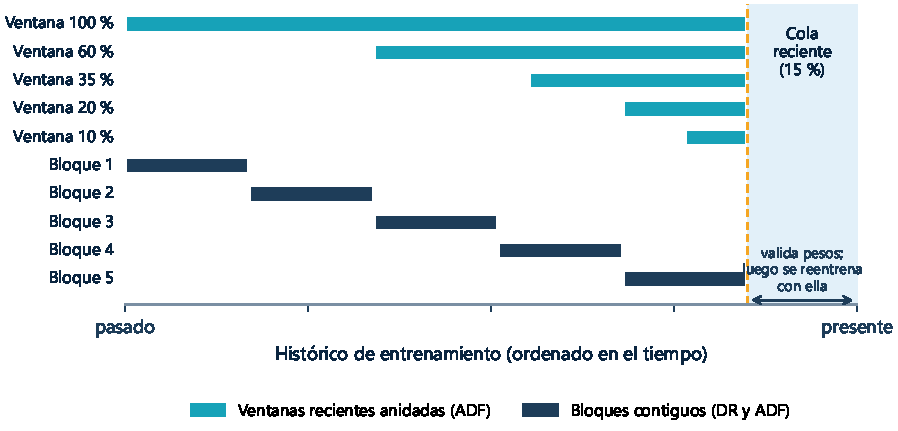
\includegraphics[width=0.95\textwidth]{figuras/candidatos.pdf}
  \caption{Modelos candidatos sobre el eje del tiempo}\label{fig:candidatos}
  \nota{Cada barra es el tramo del histórico con que se entrena un RF candidato. La cola reciente se
  usa primero para estimar los pesos y luego se incorpora al reentrenar. En el
  \texttt{DriftRegressor} en modo \texttt{mmd} no hay cola reciente y los bloques cubren todo el
  histórico.}
\end{figure}

\subsection{Líneas base}

Todos los modelos usan bosques de 100 árboles con profundidad libre, con la implementación de
scikit-learn \parencite{pedregosa2011}. Las líneas base son tres: el RF convencional entrenado con todo el
histórico, que es la referencia (RF); un RF entrenado solo con el 20\,\% más reciente, con un mínimo de
200 observaciones (RF-V); y un RF con pesos muestrales exponenciales $w_i = 0.5^{a_i/0.2}$, donde
$a_i\in[0,1)$ es la antigüedad relativa de la observación, lo que equivale a una vida media del
20\,\% del histórico (RF-E). En las tablas, DR-M, DR-R y DR-H son el \texttt{DriftRegressor} en
modos \texttt{mmd}, \texttt{recent\_error} e \texttt{hybrid}, y ADF-E y ADF-H son el
\texttt{AdaptiveDriftForest} en modos \texttt{error} e \texttt{hybrid}. DR-R+ es una variante
experimental de DR-R que reentrena el último bloque incluyendo la cola de validación; se usó para
aislar el efecto de ese cambio y solo aparece en la \cref{tab:agregado}.

\subsection{Protocolos de evaluación}

Ambos protocolos son estrictamente temporales: ningún modelo ve datos posteriores a los que predice
\parencite{tashman2000}.
\begin{itemize}
  \item Partición 80/20: entrenamiento con el primer 80\,\% y evaluación en el 20\,\% final. Es el
  protocolo de la primera versión del repositorio.
  \item Walk-forward con ventana expansiva: seis reentrenamientos con orígenes en el 40, 50, \ldots,
  90\,\% de la muestra; en cada uno se entrena con todo el pasado y se evalúa en el 10\,\% siguiente.
\end{itemize}

Los escenarios sintéticos se generan con tres semillas (0, 1 y 2); los datos reales se evalúan con la
semilla 0. La métrica principal es el cociente entre el RMSE de cada modelo y el del RF convencional
en el mismo paso y la misma semilla. Para cada conjunto de datos se resume con la media geométrica
sobre semillas y pasos, y el agregado es la media geométrica sobre conjuntos. Un cociente menor que 1
indica un error menor que el del RF. Se reportan además el número de conjuntos en que el cociente es
menor que 1, el porcentaje de pasos individuales en que el modelo gana al RF y el rango medio por
RMSE entre los nueve modelos. La significancia se evalúa con la prueba de rangos con signo de
\textcite{wilcoxon1945} sobre el logaritmo del cociente medio de cada conjunto, una observación por
conjunto, como recomienda \textcite{demsar2006} para comparar algoritmos en varios conjuntos de
datos. Con cinco conjuntos reales, el menor valor $p$ bilateral que puede alcanzar esa prueba es
$2/2^5=0.0625$, de modo que en los datos reales ninguna diferencia puede ser significativa al 5\,\%.

\subsection{Optimización de hiperparámetros}

Para comprobar que las conclusiones no dependen de la configuración por defecto, se optimizaron con
Optuna \parencite{akiba2019} tres familias (RF, RF-V y \texttt{DriftRegressor}) en diez conjuntos, con
20 ensayos por familia y validación cruzada temporal de 4 particiones (\texttt{TimeSeriesSplit})
dentro del 80\,\% de entrenamiento. El espacio de búsqueda incluye profundidad máxima (4 a 20), mínimo
de observaciones por hoja (1 a 10) y fracción de variables por división (0.5 a 1); para RF-V, la
fracción de la ventana (0.05 a 1); y para el \texttt{DriftRegressor}, $K\in\{3,\dots,8\}$,
$\beta\in[2,60]$ en escala logarítmica, el modo de ponderación, la fracción de validación (0.10 a
0.25) y $\alpha$ (0.1 a 0.9). El \texttt{AdaptiveDriftForest} no se optimizó.

\subsection{Hipótesis y criterios de veredicto}\label{sec:hipotesis}

Las hipótesis corresponden a las premisas con que se diseñó el \texttt{DriftRegressor} y a los
objetivos con que se diseñó su sucesor. Se juzgan en el protocolo walk-forward de los escenarios
sintéticos, que tiene más repeticiones, y se contrastan con los datos reales.

\begin{description}
  \item[H1.] Bajo concept drift, el \texttt{DriftRegressor} en modo \texttt{recent\_error} tiene menor
  RMSE que el RF convencional.
  \item[H2.] Cuando solo cambia $P(X)$, el \texttt{DriftRegressor} en modo \texttt{mmd} tiene menor
  RMSE que el RF convencional.
  \item[H3.] La ventaja del \texttt{DriftRegressor} proviene de la ponderación por bloques: su mejor
  modo tiene menor RMSE que las líneas base de recencia (RF-V y RF-E).
  \item[H4.] El \texttt{AdaptiveDriftForest} tiene menor RMSE que el RF convencional y que las líneas
  base de recencia, y no es peor que el RF cuando no hay concept drift.
\end{description}

Una hipótesis se considera apoyada si el cociente agregado es menor que 1 y el modelo gana en la
mayoría de los conjuntos correspondientes; apoyada en parte si se cumple solo una de las dos
condiciones o solo en un subconjunto; y no apoyada si no se cumple ninguna. Cuando el número de
conjuntos lo permite, se reporta además el valor $p$ de Wilcoxon. H4 se formuló después de observar
los resultados de H1 a H3 y se evalúa sobre los mismos conjuntos, lo que limita su alcance
(\cref{sec:limitaciones}).

% =====================================================================================
\section{Datos}\label{sec:datos}

\subsection{Escenarios sintéticos}

Los 11 escenarios sintéticos tienen 5\,000 observaciones ordenadas por un reloj normalizado
$t\in[0,1]$ y cubren los tipos de drift de la \cref{sec:marco}:

\begin{itemize}
  \item Cuatro variantes del simulador hospitalario del repositorio, con objetivo días de estancia y
  covariables edad, comorbilidades, severidad al ingreso y ocupación hospitalaria: sin drift (control),
  solo data drift (medias con tendencia y estacionalidad), solo concept drift, y ambos. El concept
  drift es una transición sigmoide entre dos funciones de estancia,
  \begin{equation}\label{eq:sigmoide}
  y_t = (1-\alpha_t)\, f_{\text{vieja}}(X_t) + \alpha_t\, f_{\text{nueva}}(X_t) + \varepsilon_t,\qquad
  \alpha_t = \frac{1}{1+\exp\{-15(t-0.6)\}}.
  \end{equation}
  \item Tres variantes de la función de \textcite{friedman1991} con diez covariables uniformes, donde el
  concepto B permuta los roles de las variables como en \textcite{ikonomovska2011}: cambio abrupto en
  $t=0.6$; cambio gradual entre $t=0.35$ y $0.75$ con data drift en cinco variables; y concepto
  recurrente A, B, A, B por cuartos, con una firma del régimen en dos covariables.
  \item Cuatro escenarios adicionales: data drift fuerte (la media de cuatro de ocho variables se
  desplaza $2\sigma$) con $P(Y\mid X)$ fijo; 20 variables correlacionadas con data drift en media y
  varianza, un cambio de signo abrupto en $t=0.7$ y un coeficiente que crece de forma incremental;
  concept drift local, que solo afecta a la región $x_0>0.6$ a partir de $t=0.55$; y coeficientes que
  rotan de forma continua.
\end{itemize}

La \cref{fig:galeria} muestra cómo se comporta cada tipo de muestra con dos indicadores simples. El
panel superior de cada escenario mide cuánto se alejan las covariables de su nivel inicial, en
desviaciones estándar del primer 30\,\%. El inferior mide el error de un modelo entrenado solo con ese
30\,\% inicial, relativo a su error dentro de ese mismo tramo: si el pasado sigue sirviendo, la
línea se queda cerca de 1.

\begin{figure}[p]
  \centering
  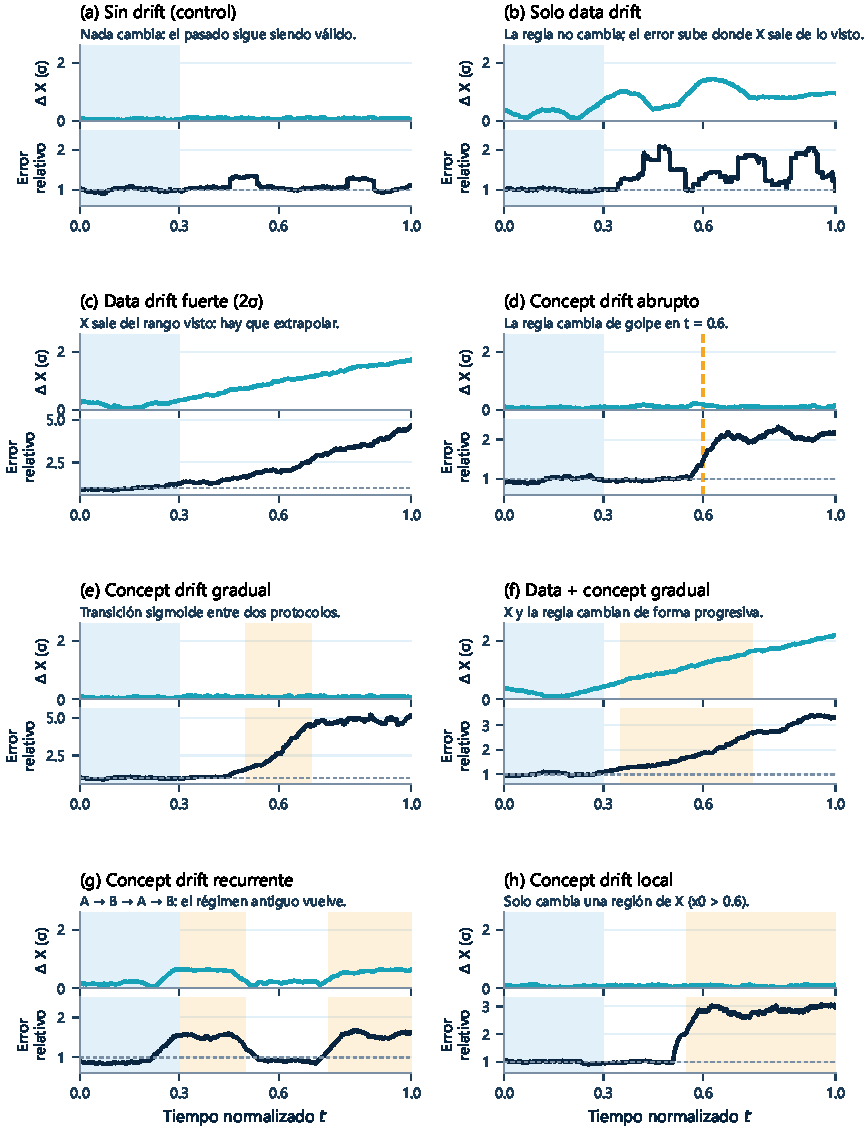
\includegraphics[width=\textwidth]{figuras/galeria_escenarios.pdf}
  \caption{Comportamiento de las muestras en ocho escenarios sintéticos}\label{fig:galeria}
  \nota{Panel superior de cada escenario: máximo, entre covariables, del valor absoluto de la media
  móvil (400 observaciones) de $X$ estandarizada con la media y la desviación del primer 30\,\%.
  Panel inferior: RMSE móvil (400 observaciones) de un RF entrenado con las filas pares del primer
  30\,\% (banda celeste), evaluado en filas que no vio y dividido por su RMSE fuera de muestra dentro
  de ese tramo; la línea punteada marca 1. Bandas y líneas naranjas: periodos en que el generador
  introduce el cambio de concepto. Semilla 0. \textit{Fuente:}
  \texttt{experiments/synthetic\_scenarios.py}.}
\end{figure}

La figura permite leer cuatro comportamientos. Sin drift (a), ambas líneas son planas: el pasado
sigue siendo válido y conviene usarlo entero. Con solo data drift (b, c), las covariables se desplazan
y el error del modelo antiguo también sube, pero no porque la regla haya cambiado, sino porque el
modelo debe predecir en zonas de $X$ que vio poco o nada. En ese caso, descartar datos antiguos no
corrige el problema, porque los datos recientes obedecen la misma regla. Con concept drift (d, e, f,
h), el error sube justo cuando cambia la regla y no vuelve a bajar, aunque $X$ no se mueva, como en
(d), (e) y (h); la MMD, que solo mira $X$, no puede verlo. Con drift recurrente (g), el error sube y
baja al ritmo en que el régimen B aparece y desaparece: es el único caso en que un modelo antiguo
vuelve a ser útil, y por eso el único en que conservar bloques del pasado tiene una ventaja
estructural.

\subsection{Datos reales}

Los cinco conjuntos reales son regresiones con drift documentado. Air Quality contiene la
concentración de CO medida por un analizador de referencia y cinco sensores químicos con deriva
conocida \parencite{devito2008}. Bike Sharing registra alquileres horarios de bicicletas en 2011 y 2012
\parencite{fanaee2014}; se excluye la variable de año para que el crecimiento del sistema actúe como
contexto oculto. Gas Sensor Drift reúne 128 rasgos de 16 sensores de gas medidos durante 36 meses
\parencite{vergara2012}; el objetivo es el logaritmo de la concentración. Beijing PM2.5 contiene la
concentración horaria de material particulado y variables meteorológicas entre 2010 y 2014
\parencite{liang2015}. Electricity (Elec2) registra la demanda eléctrica de Nueva Gales del Sur cada 30
minutos entre 1996 y 1998 \parencite{harries1999}. Beijing y Electricity se submuestrearon una de
cada tres filas para que las matrices de kernel de la MMD quepan en memoria.

\subsection{Diagnóstico de drift}

Para no depender de las etiquetas asignadas a cada conjunto, se midió el drift con cuatro indicadores
independientes de los modelos comparados (\cref{tab:datasets}). El AUC de data drift es el área bajo
la curva ROC de un bosque que distingue el 30\,\% inicial del 30\,\% final de $X$ (0.5 indica ausencia
de data drift). La ganancia de concepto (CG) es la reducción relativa del RMSE de un RF, con
validación cruzada aleatoria, al añadir el tiempo como covariable; si conocer $t$ mejora la predicción
dado $X$, entonces $P(Y\mid X)$ cambia con el tiempo. En series reales este indicador también recoge
autocorrelación de corto plazo. El cociente de recencia (RR) divide el RMSE sobre el 20\,\% final de
un RF entrenado con el primer 40\,\% entre el de uno entrenado con el tramo del 40 al 80\,\%; un valor
mayor que 1 indica que los datos antiguos predicen peor el futuro.

\begin{table}[htbp]
  \centering
  \caption{Conjuntos de datos y diagnóstico de drift}\label{tab:datasets}
  \small
  % Generado por paper/generar_tablas.py. No editar a mano.
\begin{tabularx}{\textwidth}{l X r r r r r}
\toprule
Dataset & Tipo de drift & {$n$} & {$p$} & {AUC} & {CG} & {RR} \\
\midrule
\multicolumn{7}{l}{\textit{Sintéticos (3 semillas cada uno)}} \\
\texttt{healthcare\_none} & Ninguno (control) & 5000 & 4 & 0.49 & 0.01 & 1.04 \\
\texttt{healthcare\_data} & Data & 5000 & 4 & 0.78 & 0.01 & 1.08 \\
\texttt{healthcare\_concept} & Concept gradual & 5000 & 4 & 0.49 & 0.57 & 1.81 \\
\texttt{healthcare\_both} & Data + concept & 5000 & 4 & 0.78 & 0.57 & 1.79 \\
\texttt{friedman\_abrupt} & Concept abrupto & 5000 & 10 & 0.52 & 0.25 & 1.60 \\
\texttt{friedman\_gradual\_data} & Data + concept gradual & 5000 & 10 & 0.99 & 0.06 & 1.89 \\
\texttt{friedman\_recurring} & Concept recurrente & 5000 & 10 & 0.71 & 0.04 & 1.00 \\
\texttt{covariate\_shift} & Data fuerte (2$\sigma$) & 5000 & 8 & 0.97 & -0.01 & 2.00 \\
\texttt{highdim\_mixed} & Data + concept mixto & 5000 & 20 & 0.90 & 0.33 & 1.29 \\
\texttt{local\_drift} & Concept local & 5000 & 6 & 0.50 & 0.44 & 1.83 \\
\texttt{incremental} & Concept incremental & 5000 & 10 & 0.50 & 0.03 & 1.35 \\
\addlinespace
\multicolumn{7}{l}{\textit{Reales}} \\
\texttt{air\_quality} & Deriva de sensores & 7344 & 10 & 1.00 & 0.03 & 0.95 \\
\texttt{bike\_sharing} & Contexto oculto + estacional & 17379 & 11 & 0.97 & 0.38 & 1.24 \\
\texttt{gas\_drift} & Deriva de sensores fuerte & 13910 & 134 & 1.00 & 0.01 & 1.92 \\
\texttt{beijing\_pm25} & Estacional + emisiones & 13919 & 12 & 0.82 & 0.15 & 1.02 \\
\texttt{electricity} & Mercado eléctrico & 15104 & 6 & 1.00 & 0.41 & 1.42 \\
\bottomrule
\end{tabularx}

  \nota{$n$: observaciones; $p$: covariables. AUC: área bajo la curva ROC al distinguir el 30\,\%
  inicial del final de $X$. CG: ganancia relativa de RMSE al añadir el tiempo como covariable. RR:
  cociente de recencia. En los sintéticos, diagnóstico con la semilla 0. \textit{Fuente:}
  \texttt{experiments/results/diagnostics\_*.csv}.}
\end{table}

El diagnóstico confirma el diseño de los escenarios sintéticos: los que solo tienen concept drift
muestran AUC cercano a 0.5 y CG positiva, y los que solo tienen data drift muestran AUC alto y CG
nula. En los datos reales, el AUC es cercano a 1 en cuatro de cinco conjuntos, lo que indica data
drift fuerte, mientras que la CG es alta en Bike Sharing y Electricity y casi nula en Air Quality y
Gas Drift.

% =====================================================================================
\section{Resultados}\label{sec:resultados}

\subsection{Réplica del resultado inicial}\label{sec:res-replica}

La primera versión del repositorio reportó, en el escenario hospitalario con data y concept drift y
partición 4\,000/1\,000, un RMSE de 6.40 para el RF convencional, de 5.94 para el
\texttt{DriftRegressor} en modo \texttt{mmd}, de 5.82 en modo \texttt{hybrid} y de 5.09 en modo
\texttt{recent\_error}, con $K=5$ y $\beta=15$. Con hiperparámetros optimizados por Optuna, el RMSE
pasaba de 6.39 a 4.69, una reducción del 26.6\,\%. La réplica con el código del repositorio reproduce
las cuatro primeras cifras con cuatro decimales. En modo \texttt{recent\_error} el modelo asigna
todo el peso al último bloque; en modo \texttt{mmd}, con $\beta=15$, los dos bloques más antiguos
conservan el 28\,\% del peso.

Esa comparación tiene dos límites: se hizo en el escenario más favorable para el modelo y no incluyó
ninguna línea base con recencia. Las secciones siguientes amplían la evaluación en ambas direcciones.

\subsection{DriftRegressor frente a las líneas base}\label{sec:res-dr}

La \cref{tab:sint-walk} presenta los cocientes de RMSE por escenario en el protocolo walk-forward. El
\texttt{DriftRegressor} en modo \texttt{recent\_error} mejora al RF en \hUnoGana{} de los \nConcept{}
escenarios con concept drift, con un cociente medio de \hUnoGeo{} en ese subconjunto (H1, apoyada en
parte). Sus mayores ganancias aparecen en el escenario hospitalario con concept drift
(\xDRrHealthcareConceptWalk) y en el de drift local (\xDRrLocalDriftWalk); pierde en los escenarios
con data drift fuerte y concept drift gradual o mixto.

Cuando solo hay data drift, el modo \texttt{mmd} empeora: su cociente es de \hDosMin{} en el escenario
hospitalario con data drift y de \hDosMax{} en el de data drift fuerte (H2, no apoyada). La causa es
estructural: si $P(Y\mid X)$ no cambia, cada sub-bosque estima la misma función con la quinta parte
de los datos, y la combinación de cinco estimadores con más varianza no compensa la pérdida de
muestra. Además, con $\beta=15$ los pesos quedan cerca de la uniformidad, porque los valores de
$\MMD^2$ entre bloques son del orden de 0.01 a 0.2.

\begin{table}[htbp]
  \centering
  \caption{Cociente de RMSE respecto al RF convencional, escenarios sintéticos, walk-forward}\label{tab:sint-walk}
  \small
  % Generado por paper/generar_tablas.py. No editar a mano.
\begin{tabular*}{\textwidth}{@{\extracolsep{\fill}} l rrrrrrr}
\toprule
Dataset & {RF-V} & {RF-E} & {DR-M} & {DR-R} & {DR-H} & {ADF-E} & {ADF-H} \\
\midrule
\texttt{covariate\_shift} & 1.08 & \underline{0.97} & 1.19 & 1.19 & 1.19 & 0.98 & 1.01 \\
\texttt{friedman\_abrupt} & \underline{0.82} & 0.90 & 1.04 & 0.94 & 0.99 & 0.83 & 0.83 \\
\texttt{friedman\_gradual\_data} & 0.93 & 0.97 & 1.04 & 1.11 & 1.10 & \underline{0.93} & 0.93 \\
\texttt{friedman\_recurring} & 1.02 & 1.02 & 0.98 & 0.98 & \underline{0.82} & 0.97 & 0.96 \\
\texttt{healthcare\_both} & 0.57 & 0.88 & 0.92 & 0.86 & 0.95 & \underline{0.53} & 0.55 \\
\texttt{healthcare\_concept} & 0.57 & 0.88 & 0.99 & 0.78 & 0.95 & \underline{0.52} & 0.55 \\
\texttt{healthcare\_data} & 1.11 & 1.01 & 1.18 & 1.13 & 1.29 & 1.00 & 1.05 \\
\texttt{healthcare\_none} & 1.07 & 1.01 & 0.99 & 1.01 & 1.04 & \underline{0.98} & 0.98 \\
\texttt{highdim\_mixed} & \underline{0.90} & 0.96 & 1.08 & 1.07 & 1.10 & 0.96 & 0.92 \\
\texttt{incremental} & 0.72 & 0.83 & 1.00 & 0.83 & 0.88 & \underline{0.72} & 0.74 \\
\texttt{local\_drift} & \underline{0.70} & 0.89 & 1.02 & 0.83 & 0.89 & 0.72 & 0.73 \\
\midrule
Media geométrica & 0.839 & 0.936 & 1.036 & 0.965 & 1.008 & 0.809 & 0.821 \\
\bottomrule
\end{tabular*}

  \nota{Media geométrica de RMSE$_{\text{modelo}}$/RMSE$_{\text{RF}}$ sobre 3 semillas y 6 pasos.
  Menor que 1 indica menor error que el RF. Subrayado: mejor modelo del escenario cuando mejora al RF.
  RF-V: ventana del 20\,\% reciente; RF-E: pesos exponenciales; DR-M, DR-R, DR-H:
  \texttt{DriftRegressor} en modos \texttt{mmd}, \texttt{recent\_error} e \texttt{hybrid}; ADF-E,
  ADF-H: \texttt{AdaptiveDriftForest} en modos \texttt{error} e \texttt{hybrid}. \textit{Fuente:}
  \texttt{experiments/results/benchmark\_synthetic*.csv}.}
\end{table}

La comparación con las líneas base de recencia es la que más cambia la lectura. El RF-V tiene menor
error que el mejor modo del \texttt{DriftRegressor} en \hTresRFV{} de \hTresN{} escenarios, y el RF-E
en \hTresRFE{} (H3, no apoyada). En el escenario hospitalario con ambos tipos de drift, el RF-V
alcanza un cociente de \xRFVHealthcareBothWalk{}, frente a \xDRrHealthcareBothWalk{} del mejor modo
del \texttt{DriftRegressor}. La excepción es el concept drift recurrente: ahí el modo
\texttt{hybrid} obtiene \xDRhFriedmanRecurringWalk{} y el RF-V \xRFVFriedmanRecurringWalk{}, porque
el \texttt{DriftRegressor} puede volver a dar peso a bloques antiguos cuyo régimen reaparece,
mientras que la ventana reciente solo ve el último régimen.

En los datos reales (\cref{tab:real-walk}), ningún modo del \texttt{DriftRegressor} mejora al RF de
forma consistente. El modo \texttt{mmd} gana en Electricity (\xDRmElectricityWalk) y el modo
\texttt{recent\_error} en Bike Sharing (\xDRrBikeSharingWalk), pero todos pierden en Gas Drift, donde
en la partición 80/20 el cociente llega a estar entre \gasDRmin{} y \gasDRmax{}
(\cref{tab:real-static} del \cref{app:tablas}).

\subsection{Resultados con hiperparámetros optimizados}\label{sec:res-optuna}

La \cref{tab:optuna} muestra que la optimización no cambia la conclusión. El \texttt{DriftRegressor}
optimizado mejora al RF optimizado en \optDRganaRF{} de \optN{} conjuntos, y el RF-V optimizado le gana
al \texttt{DriftRegressor} optimizado en \optRFVganaDR{} de \optN{}. En el escenario hospitalario con
ambos tipos de drift, el \texttt{DriftRegressor} reduce el RMSE del RF de \optBothRF{} a \optBothDR{}
(\optBothDRpct\,\%), pero el RF-V lo reduce a \optBothRFV{} (\optBothRFVpct\,\%). En Gas Drift, el
\texttt{DriftRegressor} optimizado tiene un error \optGasDRpct\,\% mayor que el RF. Optuna eligió
$\beta$ cercano a 57 en dos de los escenarios en modo \texttt{mmd}, lo que confirma que el valor por
defecto $\beta=15$ es bajo para la escala de la MMD.

\begin{table}[htbp]
  \centering
  \caption{RMSE en test con hiperparámetros optimizados (partición 80/20)}\label{tab:optuna}
  \small
  % Generado por paper/generar_tablas.py. No editar a mano.
\begin{tabular*}{\textwidth}{@{\extracolsep{\fill}} l r r r r l r r}
\toprule
 & \multicolumn{3}{c}{RMSE en test} & & \multicolumn{3}{c}{DR elegido por Optuna} \\
\cmidrule(lr){2-4}\cmidrule(lr){6-8}
Dataset & {RF} & {RF-V} & {DR} & {DR vs RF (\%)} & Modo & {$K$} & {$\beta$} \\
\midrule
\texttt{healthcare\_data} & \underline{1.256} & 1.330 & 1.344 & $+7.0$ & \texttt{recent\_error} & 7 & 21.5 \\
\texttt{healthcare\_both} & 6.218 & \underline{2.165} & 3.017 & $-51.5$ & \texttt{mmd} & 6 & 57.3 \\
\texttt{friedman\_abrupt} & 3.705 & \underline{3.564} & 3.724 & $+0.5$ & \texttt{mmd} & 3 & 6.7 \\
\texttt{covariate\_shift} & \underline{1.758} & 1.795 & 1.914 & $+8.9$ & \texttt{mmd} & 6 & 57.2 \\
\texttt{highdim\_mixed} & 4.971 & \underline{4.947} & 5.035 & $+1.3$ & \texttt{mmd} & 4 & 25.4 \\
\texttt{air\_quality} & 0.498 & \underline{0.482} & 0.501 & $+0.8$ & \texttt{mmd} & 3 & 32.7 \\
\texttt{bike\_sharing} & 121.80 & \underline{92.52} & 115.97 & $-4.8$ & \texttt{mmd} & 3 & 6.7 \\
\texttt{gas\_drift} & 0.605 & \underline{0.570} & 0.947 & $+56.5$ & \texttt{recent\_error} & 3 & 2.0 \\
\texttt{beijing\_pm25} & 68.34 & \underline{68.26} & 69.04 & $+1.0$ & \texttt{recent\_error} & 3 & 3.9 \\
\texttt{electricity} & 0.0762 & 0.0841 & \underline{0.0731} & $-4.0$ & \texttt{mmd} & 6 & 11.7 \\
\bottomrule
\end{tabular*}

  \nota{Optuna con 20 ensayos por familia y \texttt{TimeSeriesSplit} de 4 particiones dentro del
  80\,\% de entrenamiento. Subrayado: menor RMSE del conjunto. DR vs RF: variación porcentual del RMSE
  del \texttt{DriftRegressor} respecto al RF. $K$: número de bloques. \textit{Fuente:}
  \texttt{experiments/results/tuned\_static\_all.csv}.}
\end{table}

\subsection{AdaptiveDriftForest}\label{sec:res-adf}

La \cref{tab:agregado} resume los cuatro cortes de la evaluación. En walk-forward sintético, el
\texttt{AdaptiveDriftForest} en modo \texttt{error} tiene un cociente de \rADFeSintWalk{}, mejora al RF
en \gADFeSintWalk{} de 11 escenarios y en el \wADFeSintWalk\,\% de los pasos, con Wilcoxon
$p=\pADFeSintWalk$ y el mejor rango medio de los nueve modelos (\kADFeSintWalk). El RF-V queda en
\rRFVSintWalk{} ($p=\pRFVSintWalk$). En el subconjunto con concept drift su cociente es
\hCuatroConceptGeo{}, y en los tres escenarios sin concept drift el cociente máximo es
\hCuatroSinMax{}, de modo que ya no pierde frente al RF cuando no hay nada que adaptar. Mejora al RF-V
en \hCuatroVsRFV{} de 11 escenarios; la mayor desventaja frente a la ventana reciente aparece en el
escenario de alta dimensión (\xADFeHighdimMixedWalk{} frente a \xRFVHighdimMixedWalk).

La \cref{fig:resultados} presenta los mismos cocientes por conjunto de datos para los tres enfoques
principales. En los escenarios sintéticos, los diamantes del \texttt{AdaptiveDriftForest} quedan a
la izquierda de la línea de referencia en casi todas las filas y cerca de los puntos de la ventana
reciente, mientras que los cuadrados del \texttt{DriftRegressor} se agrupan cerca o a la derecha de
ella. En los datos reales ningún enfoque domina: el \texttt{AdaptiveDriftForest} evita las pérdidas
grandes de los otros dos (Beijing para la ventana reciente, Gas Drift para el
\texttt{DriftRegressor}), pero solo gana con claridad en Bike Sharing.

\begin{figure}[htbp]
  \centering
  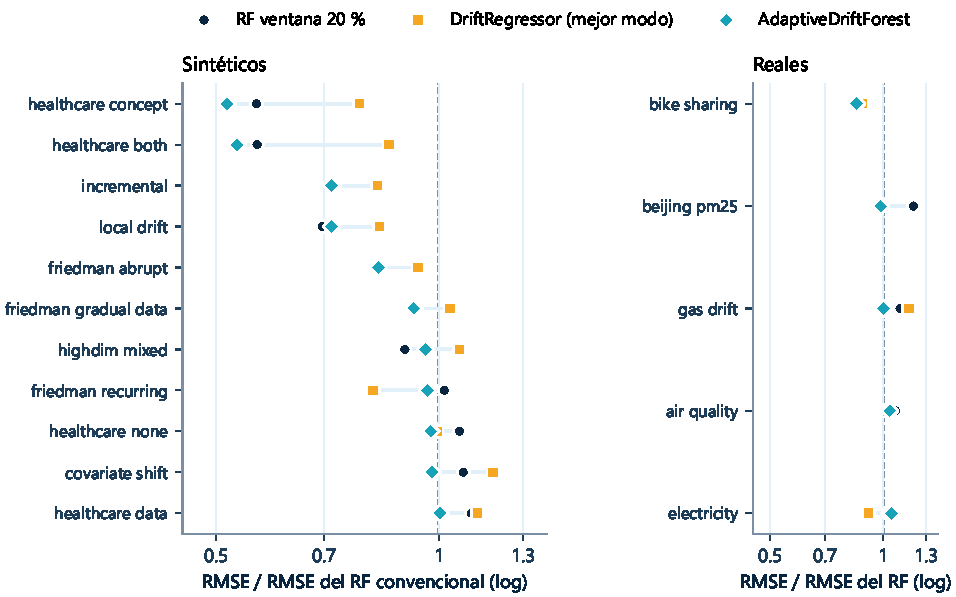
\includegraphics[width=\textwidth]{figuras/resultados_por_dataset.pdf}
  \caption{Error relativo al RF convencional por conjunto de datos (walk-forward)}\label{fig:resultados}
  \nota{Cada marcador es la media geométrica de RMSE$_{\text{modelo}}$/RMSE$_{\text{RF}}$ sobre semillas
  y pasos. A la izquierda de la línea punteada, el modelo tiene menor error que el RF. Para el
  \texttt{DriftRegressor} se muestra, en cada conjunto, su mejor modo, lo que lo favorece. Conjuntos
  ordenados por el cociente del \texttt{AdaptiveDriftForest}. \textit{Fuente:}
  \texttt{experiments/results/benchmark\_*.csv}.}
\end{figure}

\begin{table}[htbp]
  \centering
  \caption{Resumen agregado por tipo de datos y protocolo}\label{tab:agregado}
  \small
  % Generado por paper/generar_tablas.py. No editar a mano.
\begin{tabular*}{\textwidth}{@{\extracolsep{\fill}} l r c r r r}
\toprule
Modelo & {Ratio RMSE} & {Datasets $<1$} & {\% pasos $<1$} & {Rank medio} & {$p$ Wilcoxon} \\
\midrule
\multicolumn{6}{l}{\textit{Panel A. Sintéticos, walk-forward (11 escenarios $\times$ 3 semillas $\times$ 6 pasos)}} \\
ADF-E & 0.809 & 10/11 & 81 & 2.00 & 0.002 \\
ADF-H & 0.821 & 9/11 & 73 & 2.82 & 0.010 \\
RF-V & 0.839 & 7/11 & 54 & 4.00 & 0.067 \\
DR-R+ & 0.873 & 9/11 & 57 & 4.36 & 0.054 \\
RF-E & 0.936 & 8/11 & 68 & 5.09 & 0.014 \\
RF (referencia) & 1.000 & {--} & {--} & 6.09 & {--} \\
DR-R & 0.965 & 6/11 & 40 & 6.55 & 0.465 \\
DR-M & 1.036 & 5/11 & 37 & 6.91 & 0.240 \\
DR-H & 1.008 & 6/11 & 33 & 7.18 & 1.000 \\
\addlinespace
\multicolumn{6}{l}{\textit{Panel B. Sintéticos, partición 80/20 (11 escenarios $\times$ 3 semillas)}} \\
ADF-H & 0.683 & 8/11 & 79 & 2.55 & 0.014 \\
ADF-E & 0.698 & 8/11 & 79 & 2.73 & 0.042 \\
RF-V & 0.699 & 7/11 & 67 & 3.82 & 0.083 \\
DR-R+ & 0.768 & 7/11 & 64 & 4.36 & 0.175 \\
RF-E & 0.902 & 7/11 & 67 & 5.27 & 0.042 \\
RF (referencia) & 1.000 & {--} & {--} & 5.91 & {--} \\
DR-R & 0.897 & 6/11 & 52 & 6.45 & 0.278 \\
DR-H & 0.940 & 6/11 & 45 & 6.91 & 0.638 \\
DR-M & 1.019 & 4/11 & 33 & 7.00 & 0.320 \\
\addlinespace
\multicolumn{6}{l}{\textit{Panel C. Reales, walk-forward (5 datasets $\times$ 6 pasos)}} \\
ADF-E & 0.983 & 2/5 & 57 & 3.00 & 1.000 \\
RF (referencia) & 1.000 & {--} & {--} & 3.40 & {--} \\
DR-M & 1.020 & 2/5 & 40 & 4.20 & 0.625 \\
ADF-H & 1.004 & 1/5 & 50 & 4.40 & 0.625 \\
RF-E & 1.002 & 2/5 & 60 & 4.40 & 1.000 \\
DR-R+ & 1.034 & 1/5 & 33 & 5.80 & 0.625 \\
RF-V & 1.049 & 1/5 & 37 & 6.00 & 0.438 \\
DR-H & 1.088 & 0/5 & 23 & 6.40 & 0.062 \\
DR-R & 1.073 & 1/5 & 27 & 7.40 & 0.438 \\
\addlinespace
\multicolumn{6}{l}{\textit{Panel D. Reales, partición 80/20 (5 datasets)}} \\
ADF-E & 0.919 & 3/5 & 60 & 2.80 & 0.312 \\
ADF-H & 0.955 & 3/5 & 60 & 3.40 & 0.625 \\
DR-R+ & 0.961 & 2/5 & 40 & 4.00 & 1.000 \\
DR-M & 1.038 & 3/5 & 60 & 4.40 & 0.812 \\
RF (referencia) & 1.000 & {--} & {--} & 4.60 & {--} \\
DR-R & 0.990 & 2/5 & 40 & 5.60 & 1.000 \\
RF-E & 1.024 & 2/5 & 40 & 5.60 & 0.312 \\
RF-V & 1.004 & 2/5 & 40 & 6.20 & 0.812 \\
DR-H & 1.209 & 1/5 & 20 & 8.40 & 0.125 \\
\bottomrule
\end{tabular*}

  \nota{Ratio RMSE: media geométrica sobre conjuntos del cociente respecto al RF. Datasets $<1$:
  conjuntos donde el modelo mejora al RF. \% pasos $<1$: porcentaje de pares (semilla, paso) en que
  mejora al RF. Rank medio: posición media por RMSE entre los nueve modelos (1 es el mejor). $p$:
  prueba de Wilcoxon de rangos con signo sobre el log-cociente medio por conjunto. DR-R+: variante
  experimental de DR-R que reentrena el último bloque con la cola de validación. Modelos ordenados por
  rango medio. \textit{Fuente:} \texttt{experiments/results/benchmark\_*.csv}.}
\end{table}

En los datos reales la ventaja es menor. En walk-forward, el modo \texttt{error} obtiene
\rADFeRealWalk{} y es el único modelo con mejor rango medio que el RF (\kADFeRealWalk{} frente a
\kRFRealWalk); en la partición 80/20 obtiene \rADFeRealStatic{}. Ninguna de estas diferencias es
estadísticamente distinguible, como era previsible con cinco conjuntos. En Gas Drift, donde el
\texttt{DriftRegressor} perdía con claridad, el \texttt{AdaptiveDriftForest} iguala al RF
(\xADFeGasDriftWalk), porque en todos los pasos concentra la mayor parte del peso en las ventanas
largas, del 60 o del 100\,\% del histórico. En Electricity, en cambio, el
\texttt{DriftRegressor} en modo \texttt{mmd} sigue siendo mejor (\xDRmElectricityWalk{} frente a
\xADFeElectricityWalk), y en el escenario recurrente también lo es el modo \texttt{hybrid} original
(\xDRhFriedmanRecurringWalk{} frente a \xADFeFriedmanRecurringWalk).

Los pesos del \texttt{AdaptiveDriftForest} también sirven para entender qué detecta
(\cref{fig:pesos}). En el escenario con concept drift alrededor de $t=0.6$, durante los dos primeros
pasos, previos al cambio, reparte el peso entre ventanas medias y el histórico completo; desde el
paso que empieza en el 60\,\% lo concentra por completo en las ventanas cortas. En el escenario sin
drift nunca se concentra en ventanas cortas y combina ventanas largas con bloques antiguos, que en
ese caso son igual de válidos. En Gas Drift alterna entre la ventana del 60\,\% y el histórico
completo, lo que explica que iguale al RF.

\begin{figure}[htbp]
  \centering
  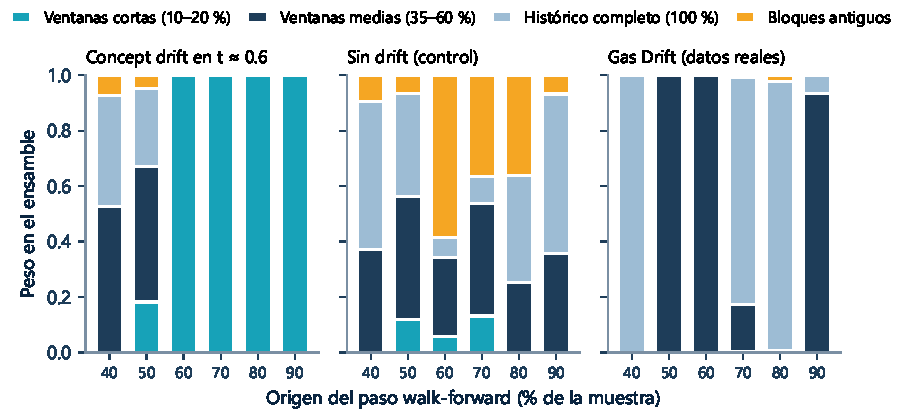
\includegraphics[width=\textwidth]{figuras/pesos_adf.pdf}
  \caption{Pesos del \texttt{AdaptiveDriftForest} en cada paso walk-forward}\label{fig:pesos}
  \nota{Peso total asignado a cada grupo de candidatos en los seis reentrenamientos (modo
  \texttt{error}, semilla 0). El eje horizontal indica el origen de cada paso como porcentaje de la
  muestra. \textit{Fuente:} \texttt{experiments/results/benchmark\_*\_adf.csv}.}
\end{figure}

La variante DR-R+, que solo añade el reentrenamiento del último bloque con la cola reciente, pasa de
\rDRrSintWalk{} a \rDRrefitSintWalk{} en walk-forward sintético. Esto aísla una parte de la mejora:
no usar los datos más recientes para entrenar era el defecto más costoso del diseño original.

\subsection{Síntesis de las hipótesis}

La \cref{tab:veredictos} contrasta cada hipótesis con el criterio fijado en la
\cref{sec:hipotesis}.

\begin{table}[htbp]
  \centering
  \caption{Contraste de hipótesis (walk-forward, escenarios sintéticos)}\label{tab:veredictos}
  \small
  \begin{tabularx}{\textwidth}{l X X l}
    \toprule
    Hip. & Lo que se esperaba & Lo que se encontró & Veredicto \\
    \midrule
    H1 & DR-R con menor RMSE que RF bajo concept drift &
      Cociente \hUnoGeo{}; gana en \hUnoGana{} de \nConcept{} escenarios & Apoyada en parte \\
    H2 & DR-M con menor RMSE que RF bajo solo data drift &
      Cocientes de \hDosMin{} y \hDosMax{}; pierde en ambos & No apoyada \\
    H3 & Mejor modo de DR con menor RMSE que RF-V y RF-E &
      RF-V gana en \hTresRFV{} de \hTresN{} y RF-E en \hTresRFE{} de \hTresN{} & No apoyada \\
    H4 & ADF con menor RMSE que RF y líneas base, sin perder sin drift &
      Cociente \rADFeSintWalk{} ($p=\pADFeSintWalk$); máximo \hCuatroSinMax{} sin concept drift; gana a
      RF-V en \hCuatroVsRFV{} de 11 & Apoyada en sintéticos \\
    \bottomrule
  \end{tabularx}
  \nota{H4 se formuló después de observar H1 a H3 y se evaluó en los mismos conjuntos (\cref{sec:limitaciones}).}
\end{table}

% =====================================================================================
\section{Discusión}\label{sec:discusion}

Los resultados indican que, en regresión por lotes, la decisión más importante ante el drift es qué
tan atrás mirar, y que esa decisión puede tomarse con un criterio tan simple como el error sobre el
tramo más reciente. El \texttt{DriftRegressor} acertaba en la dirección, porque concentraba el peso
en los bloques recientes cuando había concept drift, pero lo hacía con modelos entrenados con una
quinta parte de los datos y sin usar el tramo más reciente. El RF-V, que solo resuelve el primer
problema, ya lo superaba. El \texttt{AdaptiveDriftForest} funciona porque deja que el error reciente
elija entre ventanas de distinto largo, de modo que se comporta como un RF con todo el histórico
cuando no hay concept drift y como una ventana corta cuando lo hay.

La MMD aportó menos de lo esperado. Como solo mide cambios en $P(X)$, no distingue entre un cambio de
covariables que el modelo puede absorber y un cambio de concepto que lo invalida, y en los escenarios
de concept drift puro el diagnóstico la muestra casi nula. Su aporte aparece en dos casos: el drift
recurrente, donde el régimen deja una firma en $X$ que permite reconocer bloques antiguos útiles, y
Electricity, donde adaptar los pesos al lote de test ayuda. Ambos casos sugieren que la MMD es más
útil como criterio de selección entre modelos de regímenes ya vistos que como detector general de
drift.

Este trabajo no afirma que el \texttt{AdaptiveDriftForest} sea superior a los métodos de la
literatura de flujos de datos, con los que no se comparó, ni que su ventaja en datos reales sea
generalizable a partir de cinco conjuntos. Tampoco afirma que la ponderación por bloques carezca de
valor: el drift recurrente es un caso en el que tiene una ventaja estructural que las ventanas
recientes no pueden replicar.

\subsection{Limitaciones}\label{sec:limitaciones}

Primero, el \texttt{AdaptiveDriftForest} se diseñó después de analizar los resultados del
\texttt{DriftRegressor} en estos mismos conjuntos, de modo que su evaluación no es independiente de
su diseño. Aunque sus valores por defecto no se ajustaron a ningún conjunto, la elección de las
ventanas candidatas y de la cola de validación puede reflejar lo que funcionó aquí; su desempeño
debería confirmarse con conjuntos que no se hayan usado durante el desarrollo.

Segundo, cinco conjuntos reales no bastan para detectar diferencias moderadas con la prueba de
Wilcoxon, y los datos reales se evaluaron con una sola semilla.

Tercero, la búsqueda de hiperparámetros usó 20 ensayos por familia y no incluyó al
\texttt{AdaptiveDriftForest}; una búsqueda más amplia podría cambiar la distancia entre modelos.

Cuarto, la ganancia de concepto en series reales también recoge autocorrelación de corto plazo, por
lo que sobreestima el concept drift en datos con alta frecuencia temporal.

Quinto, el \texttt{AdaptiveDriftForest} entrena cerca del doble de bosques que el
\texttt{DriftRegressor}; en Gas Drift, con 134 covariables, cada ajuste tarda alrededor de 90
segundos.

% =====================================================================================
\section{Conclusiones}\label{sec:conclusiones}

Bajo concept drift, el \texttt{DriftRegressor} mejora al bosque aleatorio convencional en la mayoría
de los escenarios sintéticos, aunque no en todos (P1).

Cuando solo cambia la distribución de las covariables, el \texttt{DriftRegressor} es peor que el
bosque convencional, porque divide la muestra sin corregir ningún sesgo (P2).

La ventaja del \texttt{DriftRegressor} se explica sobre todo por la recencia: un bosque entrenado con
el 20\,\% más reciente del histórico lo supera en la mayoría de los escenarios. La ponderación por
bloques solo aporta algo propio en el drift recurrente (P3).

El \texttt{AdaptiveDriftForest}, al incluir ventanas recientes anidadas entre sus candidatos y
reentrenar con los datos más nuevos, es el modelo con mejor rango medio en los cuatro cortes evaluados
y no pierde frente al bosque convencional cuando no hay drift. Su ventaja es clara en los datos
sintéticos y modesta, sin significancia estadística, en los reales (P4).

% =====================================================================================
\section{Recomendaciones}\label{sec:recomendaciones}

\subsection{Para quien modela datos con drift}

Diagnosticar antes de elegir el modelo. Los tres indicadores de la \cref{tab:datasets} (AUC de data
drift, ganancia de concepto y cociente de recencia) se calculan en minutos y separan los casos de la
\cref{fig:galeria}. Un AUC alto con ganancia de concepto nula, como en los escenarios de solo data
drift y en Gas Drift, sugiere conservar el histórico completo; una ganancia de concepto alta junto con
un cociente de recencia alto sugiere probar primero la recencia. Los indicadores orientan, pero no
reemplazan la evaluación walk-forward: en el escenario incremental la ganancia de concepto es baja
(0.03) y, aun así, la ventana reciente reduce el error en cerca de 30\,\%.

Evaluar siempre con validación temporal. La validación cruzada aleatoria mezcla el futuro con el
pasado y oculta el drift; el protocolo walk-forward reproduce la forma en que el modelo se usará:
reentrenarlo cada cierto tiempo y predecir el tramo siguiente.

Incluir líneas base de recencia. Un RF con el 20\,\% más reciente y un RF con pesos exponenciales
cuestan lo mismo que el RF convencional y, en este trabajo, superaron al método adaptativo original.
Un método que no les gana no justifica su complejidad.

Reentrenar con los datos más recientes. Reservar el tramo final solo para validar y no usarlo después
para entrenar fue el defecto más costoso del diseño original; los datos más nuevos son los más
informativos cuando hay concept drift.

Vigilar los pesos, no solo el error. En el \texttt{AdaptiveDriftForest}, un desplazamiento del peso
hacia las ventanas cortas (\cref{fig:pesos}) indica que el pasado dejó de servir. Esa señal puede
usarse como alerta de cambio en un sistema en producción.

\subsection{Para el desarrollo del modelo en el CCDE}

Usar el \texttt{AdaptiveDriftForest} como modelo principal y conservar el \texttt{DriftRegressor}
solo como referencia, hasta que su modo \texttt{mmd} admita predicciones de una fila y deje de
depender del lote. Actualizar la documentación del repositorio para que toda cifra de mejora se
reporte junto a las líneas base de recencia y en ambos protocolos. Mantener el banco de pruebas de
este trabajo (escenarios, conjuntos reales, protocolos y diagnóstico) como estándar mínimo para
evaluar cualquier variante nueva.

% =====================================================================================
\section{Trabajo futuro}\label{sec:futuro}

Las líneas siguientes se ordenan de menor a mayor esfuerzo. Las tres primeras atienden limitaciones
de este trabajo; las demás extienden el método.

\begin{description}
  \item[Validación externa.] Evaluar el \texttt{AdaptiveDriftForest} en conjuntos que no se usaron
  durante su diseño, con el protocolo y las hipótesis fijados antes de ver los resultados. Las series
  económicas y financieras con cambios estructurales documentados son candidatas naturales para el
  CCDE.
  \item[Selección de pesos más estable.] Estimar los pesos con varios cortes recientes en lugar de
  uno, para reducir la varianza de la elección cuando la cola de validación es corta, y optimizar con
  Optuna $\beta$, las fracciones de ventana y el tamaño de la cola.
  \item[Más evidencia en datos reales.] Ampliar el número de conjuntos reales y de semillas para que
  la prueba de Wilcoxon tenga potencia, y comparar contra métodos de flujos de datos como Adaptive
  Random Forests \parencite{gomes2017}, disponibles en bibliotecas como River
  \parencite{montiel2021}.
  \item[Memoria de regímenes.] Combinar las ventanas del \texttt{AdaptiveDriftForest} con la capacidad
  del \texttt{DriftRegressor} de recuperar bloques antiguos: cuando la MMD entre la cola reciente y un
  bloque antiguo sea baja y su error reciente también, reactivar ese bloque. Es el caso de la
  \cref{fig:galeria}(g), donde la versión original todavía gana.
  \item[Adaptación al lote como opción.] Ofrecer un modo que ajuste los pesos al lote que se va a
  predecir, útil en casos como Electricity, sin perder la predicción fila a fila del modo por
  defecto.
  \item[Detección explícita del cambio.] Acoplar un detector de cambio, como ventanas adaptativas
  \parencite{bifet2007} o pruebas de cambio estructural \parencite{baiperron1998}, para decidir
  cuándo reentrenar en lugar de hacerlo a intervalos fijos.
  \item[Bootstrap temporal probabilístico.] Reemplazar el bootstrap uniforme de cada árbol por uno
  que muestree con probabilidad $w_i \propto e^{-\alpha\,\Delta t_i}$, controlando el tamaño efectivo
  de muestra para no perder demasiada información.
  \item[Divisiones de árbol sensibles al drift.] Añadir al criterio de división de los primeros
  niveles un término que penalice separar regiones con distribuciones distintas en el tiempo, con la
  MMD aproximada mediante características aleatorias de Fourier \parencite{rahimi2007} para que el
  costo sea manejable.
  \item[Intervalos de predicción.] Acompañar cada predicción con un intervalo válido bajo drift,
  usando predicción conformal con ponderación temporal \parencite{barber2023}; en aplicaciones de
  riesgo, el ancho del intervalo es tan importante como el punto.
  \item[Clasificación y paquete instalable.] Extender el método a clasificación y empaquetarlo con
  pruebas automáticas y documentación para que otros miembros del CCDE lo usen en sus proyectos.
\end{description}

\printbibliography[title={Referencias}]

% =====================================================================================
\appendix
\section{Tablas complementarias}\label{app:tablas}

\begin{table}[htbp]
  \centering
  \caption{Cociente de RMSE respecto al RF convencional, datos reales, walk-forward}\label{tab:real-walk}
  \small
  % Generado por paper/generar_tablas.py. No editar a mano.
\begin{tabular*}{\textwidth}{@{\extracolsep{\fill}} l rrrrrrr}
\toprule
Dataset & {RF-V} & {RF-E} & {DR-M} & {DR-R} & {DR-H} & {ADF-E} & {ADF-H} \\
\midrule
\texttt{air\_quality} & 1.08 & 1.03 & 1.03 & 1.06 & 1.03 & 1.04 & 1.01 \\
\texttt{beijing\_pm25} & 1.20 & 1.01 & 0.99 & 1.08 & 1.06 & \underline{0.98} & 1.03 \\
\texttt{bike\_sharing} & 0.86 & 0.97 & 1.01 & 0.88 & 1.05 & \underline{0.85} & 0.91 \\
\texttt{electricity} & 1.03 & 0.98 & \underline{0.91} & 1.13 & 1.06 & 1.05 & 1.06 \\
\texttt{gas\_drift} & 1.11 & 1.01 & 1.17 & 1.25 & 1.26 & 1.00 & 1.01 \\
\midrule
Media geométrica & 1.049 & 1.002 & 1.020 & 1.073 & 1.088 & 0.983 & 1.004 \\
\bottomrule
\end{tabular*}

  \nota{Media geométrica sobre 6 pasos, semilla 0. Abreviaturas como en la \cref{tab:sint-walk}.
  \textit{Fuente:} \texttt{experiments/results/benchmark\_real*.csv}.}
\end{table}

\begin{table}[htbp]
  \centering
  \caption{Cociente de RMSE respecto al RF convencional, escenarios sintéticos, partición 80/20}\label{tab:sint-static}
  \small
  % Generado por paper/generar_tablas.py. No editar a mano.
\begin{tabular*}{\textwidth}{@{\extracolsep{\fill}} l rrrrrrr}
\toprule
Dataset & {RF-V} & {RF-E} & {DR-M} & {DR-R} & {DR-H} & {ADF-E} & {ADF-H} \\
\midrule
\texttt{covariate\_shift} & 1.08 & 1.00 & 1.17 & 1.25 & 1.23 & 1.00 & 1.02 \\
\texttt{friedman\_abrupt} & \underline{0.56} & 0.78 & 0.99 & 0.74 & 0.87 & 0.62 & 0.58 \\
\texttt{friedman\_gradual\_data} & 0.93 & 0.98 & 1.02 & 1.18 & 1.18 & 0.92 & \underline{0.92} \\
\texttt{friedman\_recurring} & 1.15 & 1.01 & 1.01 & 1.13 & \underline{0.72} & 1.02 & 1.01 \\
\texttt{healthcare\_both} & 0.32 & 0.85 & 0.89 & 0.76 & 0.85 & 0.29 & \underline{0.29} \\
\texttt{healthcare\_concept} & 0.36 & 0.80 & 1.00 & 0.62 & 0.76 & \underline{0.31} & 0.33 \\
\texttt{healthcare\_data} & 1.03 & 1.01 & 1.12 & 1.11 & 1.16 & \underline{0.98} & 1.02 \\
\texttt{healthcare\_none} & 1.08 & 1.01 & 0.98 & 0.99 & 1.01 & \underline{0.97} & 0.97 \\
\texttt{highdim\_mixed} & \underline{0.71} & 0.92 & 1.05 & 1.10 & 1.34 & 1.09 & 0.80 \\
\texttt{incremental} & \underline{0.67} & 0.80 & 0.99 & 0.80 & 1.00 & 0.67 & 0.71 \\
\texttt{local\_drift} & \underline{0.50} & 0.80 & 1.01 & 0.54 & 0.55 & 0.52 & 0.51 \\
\midrule
Media geométrica & 0.699 & 0.902 & 1.019 & 0.897 & 0.940 & 0.698 & 0.683 \\
\bottomrule
\end{tabular*}

  \nota{Media geométrica sobre 3 semillas. Abreviaturas como en la \cref{tab:sint-walk}.
  \textit{Fuente:} \texttt{experiments/results/benchmark\_synthetic*.csv}.}
\end{table}

\begin{table}[htbp]
  \centering
  \caption{Cociente de RMSE respecto al RF convencional, datos reales, partición 80/20}\label{tab:real-static}
  \small
  % Generado por paper/generar_tablas.py. No editar a mano.
\begin{tabular*}{\textwidth}{@{\extracolsep{\fill}} l rrrrrrr}
\toprule
Dataset & {RF-V} & {RF-E} & {DR-M} & {DR-R} & {DR-H} & {ADF-E} & {ADF-H} \\
\midrule
\texttt{air\_quality} & 0.98 & 1.04 & 0.94 & 0.92 & 0.98 & 0.90 & \underline{0.89} \\
\texttt{beijing\_pm25} & 1.14 & 0.98 & 1.01 & 1.06 & 1.09 & \underline{0.97} & 1.04 \\
\texttt{bike\_sharing} & 0.72 & 0.99 & 0.98 & \underline{0.63} & 1.03 & 0.74 & 0.85 \\
\texttt{electricity} & 1.07 & 1.02 & \underline{0.91} & 1.04 & 1.23 & 1.01 & 1.02 \\
\texttt{gas\_drift} & 1.20 & 1.09 & 1.43 & 1.50 & 1.89 & 1.00 & \underline{0.99} \\
\midrule
Media geométrica & 1.004 & 1.024 & 1.038 & 0.990 & 1.209 & 0.919 & 0.955 \\
\bottomrule
\end{tabular*}

  \nota{Semilla 0. Abreviaturas como en la \cref{tab:sint-walk}. \textit{Fuente:}
  \texttt{experiments/results/benchmark\_real*.csv}.}
\end{table}

\section{Reproducibilidad}\label{app:repro}

El código y los resultados están en el repositorio \texttt{DriftAdaptiveForest}, rama
\texttt{mejoras-modelo-drift}, con Python 3, scikit-learn, SciPy y Optuna (versiones en
\texttt{requirements.txt}). Desde la raíz del repositorio:

\begin{verbatim}
python -I experiments/benchmark_drift.py --suite all --seeds 0 1 2
python -I experiments/benchmark_drift.py --suite all --seeds 0 1 2 \
       --models ADF_error ADF_hybrid --no-diag --tag adf
python -I experiments/tune_benchmark.py --trials 20
python -I experiments/summarize_benchmark.py
python paper/generar_tablas.py
\end{verbatim}

El último comando reescribe las tablas y las cifras del texto (\texttt{paper/tablas/}) a partir de
los archivos de resultados, de modo que el documento se mantiene coherente con ellos.

\end{document}
